% main.tex -- computation-suite article (fea_engine + rom_engine).
% Build: pdflatex main && bibtex main && pdflatex main && pdflatex main
% Numbers in the text are macros from tables/numbers.tex, generated by experiments/make_tables.py.
\documentclass[11pt,a4paper]{article}
% macros.tex -- preamble shared by main.tex.
\usepackage[T1]{fontenc}
\usepackage[utf8]{inputenc}
\usepackage{lmodern}
\usepackage[margin=2.5cm]{geometry}
\usepackage{amsmath,amssymb,bm}
\usepackage{graphicx}
\usepackage{booktabs,array}
\usepackage{xcolor}
\usepackage{enumitem}
\usepackage{microtype}
\usepackage{listings}
\usepackage{float}
\usepackage{tikz}
\usetikzlibrary{positioning,fit,arrows.meta,calc,backgrounds}
\usepackage[numbers,sort&compress]{natbib}
\usepackage[colorlinks=true,linkcolor=blue!50!black,citecolor=blue!50!black,urlcolor=blue!50!black]{hyperref}
\usepackage[capitalise,noabbrev]{cleveref}

% generated numbers (see experiments/make_tables.py)
% generated by make_tables.py -- do not edit
\newcommand{\elasticaN}{40}
\newcommand{\elasticaWerr}{$3.5\times10^{-6}$}
\newcommand{\elasticaShortErr}{$2.2\times10^{-4}$}
\newcommand{\elasticaWref}{0.301721}
\newcommand{\elasticaShortRef}{0.056433}
\newcommand{\patchMaxErr}{$2\times10^{-14}$}
\newcommand{\quadBendingMaxErr}{$8\times10^{-13}$}
\newcommand{\eOneElements}{120}
\newcommand{\eOneFull}{242}
\newcommand{\eOneReduced}{10}
\newcommand{\eOneErr}{$1.5\times10^{-3}$}
\newcommand{\eOneSpeedup}{254}
\newcommand{\eOneSweep}{500}
\newcommand{\eOneTfom}{1812}
\newcommand{\eOneTrom}{7.1}
\newcommand{\cmsFullSize}{78}
\newcommand{\recoveryMinSpeedup}{23}
\newcommand{\recoveryMaxSpeedup}{53}
\newcommand{\recoveryLoopMsMin}{0.21}
\newcommand{\recoveryLoopMsMax}{0.75}
\newcommand{\recoveryLoopMax}{4000}
\newcommand{\recoveryBigElements}{10000}
\newcommand{\recoveryBigMs}{42}
\newcommand{\torchAvailable}{1}
\newcommand{\torchVersion}{2.7.0+cu126}
\newcommand{\torchGpu}{NVIDIA GeForce GTX 1050}
\newcommand{\torchCuda}{12.6}
\newcommand{\torchDriver}{532.09}
\newcommand{\torchHasGpu}{1}
\newcommand{\torchMaxDiff}{$1\times10^{-12}$}
\newcommand{\torchOs}{Windows}
\newcommand{\torchCpus}{12}
\newcommand{\torchPython}{3.10.18}
\newcommand{\torchNumpy}{1.26.4}
\newcommand{\torchScipy}{1.15.3}
\newcommand{\torchCommit}{ac90d0b}
\newcommand{\torchCrossCpu}{16640}
\newcommand{\torchCrossGpu}{66048}
\newcommand{\torchStressCrossCpuElems}{8192}
\newcommand{\torchStressCrossGpuElems}{8192}
\newcommand{\torchBigDof}{66048}
\newcommand{\torchBigScipyMs}{2070.4}
\newcommand{\torchBigCpuMs}{2284.7}
\newcommand{\torchBigCpuRatio}{0.91}
\newcommand{\torchBigStressNumpyMs}{165.7}
\newcommand{\torchBigStressCpuMs}{70.8}
\newcommand{\torchBigGpuMs}{836.0}
\newcommand{\torchBigGpuRatio}{2.48}
\newcommand{\torchBigStressGpuMs}{47.7}
\newcommand{\feaLines}{27\,061}
\newcommand{\romLines}{13\,196}
\newcommand{\totalLines}{40\,257}
\newcommand{\feaFiles}{50}
\newcommand{\romFiles}{38}
\newcommand{\feaTestLines}{22\,250}
\newcommand{\romTestLines}{11\,348}
\newcommand{\feaTests}{1\,144}
\newcommand{\romTests}{463}
\newcommand{\nElements}{29}
\newcommand{\nConstitutive}{6}
\newcommand{\feaPublic}{142}
\newcommand{\romPublic}{117}
\newcommand{\feaVersion}{1.0.1}
\newcommand{\romVersion}{0.2.0}
\newcommand{\qsDof}{650}
\newcommand{\qsFree}{624}
\newcommand{\qsModes}{8}
\newcommand{\qsTip}{$1.797\times10^{-4}$}
\newcommand{\qsErr}{$1\times10^{-15}$}
\newcommand{\envPython}{3.10.12}
\newcommand{\envCpus}{2}
\newcommand{\envNumpy}{2.2.6}
\newcommand{\envScipy}{1.15.3}
\newcommand{\envCommit}{ac90d0b}
\newcommand{\eOneMeanErr}{$5.6\times10^{-4}$}
\newcommand{\eOneNtest}{8}
\newcommand{\eOneNtrain}{10}
\newcommand{\ebFirstHz}{20.951}
\newcommand{\ebRelErrTwenty}{$5.4\times10^{-8}$}
\newcommand{\timoRelErr}{$9.7\times10^{-4}$}
\newcommand{\timoN}{4}
\newcommand{\quadBendFine}{0.9922}
\newcommand{\triBendFine}{0.9479}
\newcommand{\cmsFirstHz}{533.3}
\newcommand{\cmsErrTwo}{$3.2\times10^{-3}$}
\newcommand{\cmsSizeTwo}{6}
\newcommand{\cmsErrFive}{$9.3\times10^{-5}$}
\newcommand{\cmsSizeFive}{12}
\newcommand{\cmsErrAll}{$5.2\times10^{-11}$}
\newcommand{\cmsSizeAll}{78}
\newcommand{\ecswBigKept}{16}
\newcommand{\ecswBigTotal}{120}
\newcommand{\ecswBigForceSpeed}{9.4}
\newcommand{\ecswBigTrajSpeed}{7.3}
\newcommand{\ecswBigTrajErr}{$4.5\times10^{-5}$}
\newcommand{\ecswBigForceErr}{$1.2\times10^{-4}$}
\newcommand{\ecswSteps}{300}
\newcommand{\ecswModes}{3}
\newcommand{\wfFirstHz}{897}
\newcommand{\wfVmMax}{62}
\newcommand{\wfErr}{$7.0\times10^{-5}$}
\newcommand{\wfPassed}{passed}
\newcommand{\resultsGenerated}{yes}


% code listings
\lstdefinestyle{py}{language=Python,basicstyle=\ttfamily\footnotesize,keywordstyle=\color{blue!60!black},
  commentstyle=\color{green!40!black},stringstyle=\color{red!50!black},showstringspaces=false,
  frame=single,framerule=0.3pt,rulecolor=\color{black!30},xleftmargin=2pt,xrightmargin=2pt,
  breaklines=true,columns=fullflexible,keepspaces=true}
\lstset{style=py,captionpos=b}
\usepackage[font=small,labelfont=bf]{caption}\captionsetup{justification=raggedright,singlelinecheck=false}

% notation
\newcommand{\K}{\bm{K}}
\newcommand{\M}{\bm{M}}
\newcommand{\C}{\bm{C}}
\newcommand{\F}{\bm{F}}
\newcommand{\vu}{\bm{u}}
\newcommand{\pkg}[1]{\texttt{#1}}
\newcommand{\fea}{\pkg{fea\_engine}}
\newcommand{\rom}{\pkg{rom\_engine}}
\newcommand{\fint}{\bm{f}_{\mathrm{int}}}
\newcommand{\fext}{\bm{f}_{\mathrm{ext}}}
\newcommand{\KT}{\K_{\mathrm{T}}}
\newcommand{\Mat}[1]{\mathbf{#1}}
% Set to the Zenodo DOI after archiving the release, e.g. \renewcommand{\zenodoDoi}{10.5281/zenodo.1234567}
\newcommand{\zenodoDoi}{}\newcommand{\noDoi}{}
\newcommand{\todo}[1]{\textcolor{red}{\textbf{[TODO: #1]}}}
\emergencystretch=2em

% Pseudocode: self-contained, so the paper does not depend on algorithm.sty / algpseudocode.sty being installed.
\floatstyle{ruled}\newfloat{algorithm}{tbp}{loa}\floatname{algorithm}{Algorithm}
\newcounter{algline}\newdimen\algindent\newdimen\algtmp
\newenvironment{algorithmic}[1][]{\par\small\setcounter{algline}{0}\algindent=0pt\relax}{\par\smallskip}
\newcommand{\State}{\par\noindent\stepcounter{algline}\algtmp=\algindent\advance\algtmp by 1.8em \hangindent=\algtmp \hangafter=1
  \hspace*{\algindent}\makebox[1.8em][l]{\scriptsize\thealgline:}}
\newcommand{\Require}{\par\noindent\hangindent=1.8em \hangafter=1 \textbf{Require:}\ }
\newcommand{\Comment}[1]{\hfill$\triangleright$ #1}
\newcommand{\For}[1]{\State\textbf{for} #1 \textbf{do}\global\advance\algindent by 1.4em\relax}
\newcommand{\EndFor}{\global\advance\algindent by -1.4em\relax\State\textbf{end for}}


\title{A verification-first Python toolkit for structural finite element analysis\\
and reduced-order modelling: \texttt{fea\_engine} and \texttt{rom\_engine}}
\author{Abhijeet Kumar\\[2pt]
{\small [affiliation to be supplied]}\\
{\small \texttt{[e-mail to be supplied]}}}
\date{\today}

\begin{document}
\maketitle

\begin{abstract}
Structural analysis with the finite element method (FEM) and model order reduction (MOR) are usually done in separate software.
We describe \texttt{computation-suite}, two MIT-licensed Python packages, \fea{} and \rom{}, that depend only on NumPy and SciPy and keep both steps in one code base.
\fea{} provides \nElements{} element formulations (trusses, beams, plane and solid continua, plates, shells, contact), linear, modal, harmonic, transient and nonlinear analyses, exact elimination of linear constraints, and batched or differentiable (PyTorch) stress recovery.
\rom{} works on plain stiffness, mass and load arrays and provides POD--Galerkin and affine parametric models with error bounds, Krylov and balanced-truncation methods, Craig--Bampton synthesis, ECSW and DEIM hyper-reduction, and surrogate and harmonic-balance nonlinear models.
We state the formulations and algorithms and compare the results with closed-form and independent references: patch tests pass to rounding error, and observed convergence orders agree with theory.
On one 2-core CPU, an affine POD--Galerkin model answers a 500-query parameter sweep \eOneSpeedup{} times faster than dense full-order solves, with a held-out error of \eOneErr{}, and batched stress recovery is \recoveryMinSpeedup{} to \recoveryMaxSpeedup{} times faster than the element loop.
The paper also lists the limits of the current implementation, and every number in it is regenerated by scripts in the repository.
\end{abstract}

\noindent\textbf{Keywords:} finite element method, model order reduction, structural mechanics, Python, open-source software,
verification.

\section{Introduction}\label{sec:intro}

The finite element method (FEM) is the standard tool for structural analysis \cite{zienkiewicz2013fem,bathe2014fep}.
Its cost grows with the number of degrees of freedom (DOF), and many-query tasks such as parameter studies, design
optimisation, uncertainty quantification and real-time prediction need the same model solved many times.
Model order reduction (MOR) addresses this by replacing the full model with a small one built from a projection basis
\cite{benner2015survey,hesthaven2016rb,antoulas2005}.
In practice the two steps live in different software: one tool assembles and solves the full model, another builds the
reduced model, and the user moves matrices between them.

This paper describes \texttt{computation-suite}, an open-source collection of two Python packages that keep both steps
in one code base while keeping them decoupled:

\begin{itemize}[leftmargin=*,itemsep=2pt]
  \item \fea{} (version~\feaVersion{}) is a finite element package for structural mechanics. It registers \nElements{}
  element formulations and \nConstitutive{} constitutive models and provides static, modal, harmonic, transient and
  nonlinear analyses (\cref{sec:arch}).
  \item \rom{} (version~\romVersion{}) works on plain arrays $\K,\M,\C,\F$. It includes projection-based, state-space,
  surrogate-based and hyper-reduction methods and component mode synthesis, and can be used on matrices that come from any
  other source.
\end{itemize}

Both depend only on NumPy \cite{harris2020numpy} and SciPy \cite{virtanen2020scipy}. PyTorch \cite{paszke2019pytorch} is an optional
backend for GPU solves and differentiable stress recovery.
The library code has \totalLines{} lines (\feaLines{} in \fea{}, \romLines{} in \rom{}) and is checked by \feaTests{} and
\romTests{} automated tests.

\paragraph{Contributions.}
The paper (i) documents the architecture and the interfaces between the FE and ROM layers;
(ii) states the mathematics and algorithms behind the main components, with references to the original methods;
(iii) reports verification against closed-form and independent reference solutions, including observed convergence orders;
(iv) reports speed-ups of reduced and batched computations measured by scripts that ship with the repository, so the numbers
can be reproduced; and (v) states the known limitations. We make no claim that the package is faster than, or replaces,
established libraries; \cref{sec:related} places it among them.

\paragraph{Outline.}
\Cref{sec:related} reviews related software and \cref{sec:arch} describes the package structure and interfaces. \Cref{sec:fe,sec:constraints,sec:analysis,sec:nonlinear,sec:recovery} give the finite element formulation, constraints, linear and nonlinear analyses and derived results;
\cref{sec:rom} gives the reduction methods. \Cref{sec:verif,sec:perf} report verification and performance, \cref{sec:usage} shows a workflow, and \cref{sec:limits,sec:avail} state limitations and availability.

\section{Related work}\label{sec:related}

\paragraph{Finite element software.}
General-purpose open-source finite element libraries with Python interfaces include FEniCS/DOLFINx \cite{logg2012fenics,baratta2023dolfinx},
MFEM \cite{anderson2021mfem}, Kratos Multiphysics \cite{dadvand2010kratos}, scikit-fem \cite{gustafsson2020skfem} and SfePy \cite{cimrman2019sfepy}.
OpenSeesPy \cite{zhu2018openseespy} exposes the OpenSees framework for structural and earthquake engineering from Python.
The first group is organised around weak forms and generic discretisation, the last around ready-made structural elements.
Recently, finite element tooling built natively on PyTorch has also appeared: the TensorMesh library \cite{tensormesh2026} and the TensorGalerkin assembly algorithm of Wen et al.\ \cite{wen2026tensorgalerkin}.
\fea{} follows the structural-element tradition: elements are classes with explicit $\bm B$-matrices and stiffness, mass and internal-force
methods rather than forms assembled from a variational language.

\paragraph{Model order reduction software.}
pyMOR \cite{milk2016pymor} is a mature Python library for reduced-basis and related methods, designed around abstract operator
interfaces and parameterised models. \rom{} takes a smaller route: methods act on explicit matrices and vectors, and the
FE side only has to supply them. The methods themselves are established; \cref{sec:rom} gives the references.

\paragraph{Scope comparison.}
\Cref{tab:scope} lists the focus of each package in qualitative terms, taken from the cited publications. It does not rank the packages
and says nothing about performance.

\begin{table}[t]
\centering\footnotesize
\caption{Qualitative scope of related software, as described in the cited publications. The last row is this work.}
\label{tab:scope}
\begin{tabular}{>{\raggedright\arraybackslash}p{2.9cm}>{\raggedright\arraybackslash}p{3.4cm}>{\raggedright\arraybackslash}p{3.9cm}>{\raggedright\arraybackslash}p{3.6cm}}
\toprule
Package & Core idea & Typical use & Reduction methods \\
\midrule
FEniCS/DOLFINx \cite{logg2012fenics,baratta2023dolfinx} & automated solution of PDEs from weak forms & general PDE problems & not part of the core \\
MFEM \cite{anderson2021mfem} & scalable high-order finite elements, C++ with Python bindings & large-scale parallel simulation & not part of the core \\
Kratos \cite{dadvand2010kratos} & multi-physics framework & coupled multi-physics & separate application modules, including reduced-order work (not assessed here) \\
scikit-fem \cite{gustafsson2020skfem} & assembly of weak forms in NumPy/SciPy & research prototypes & not part of the core \\
SfePy \cite{cimrman2019sfepy} & problem description files, weak forms & general PDE problems & homogenisation, not a MOR suite \\
OpenSeesPy \cite{zhu2018openseespy} & structural-engineering framework with Python interface & structural and earthquake analysis & not part of the core \\
pyMOR \cite{milk2016pymor} & abstract operator interface for reduction & parametric reduced-basis models & reduced-basis, balanced truncation and others \\
\midrule
\fea{} + \rom{} & structural elements and ROMs on explicit arrays & structural FE with reduction in one place & \cref{sec:rom} \\
\bottomrule
\end{tabular}
\end{table}

\section{Software architecture}\label{sec:arch}

\subsection{Package layout}
The repository contains two independently installable packages (\cref{fig:arch}).
\fea{} has \feaFiles{} source files and \rom{} has \romFiles{} (counts from \texttt{experiments/e0\_inventory.py}).
The public API exports \feaPublic{} names from \fea{} and \romPublic{} from \rom{}.
\rom{} does not import \fea{}; the only contract between them is the set of plain arrays that
\texttt{FESystem} exposes.

\begin{figure}[t]
\centering
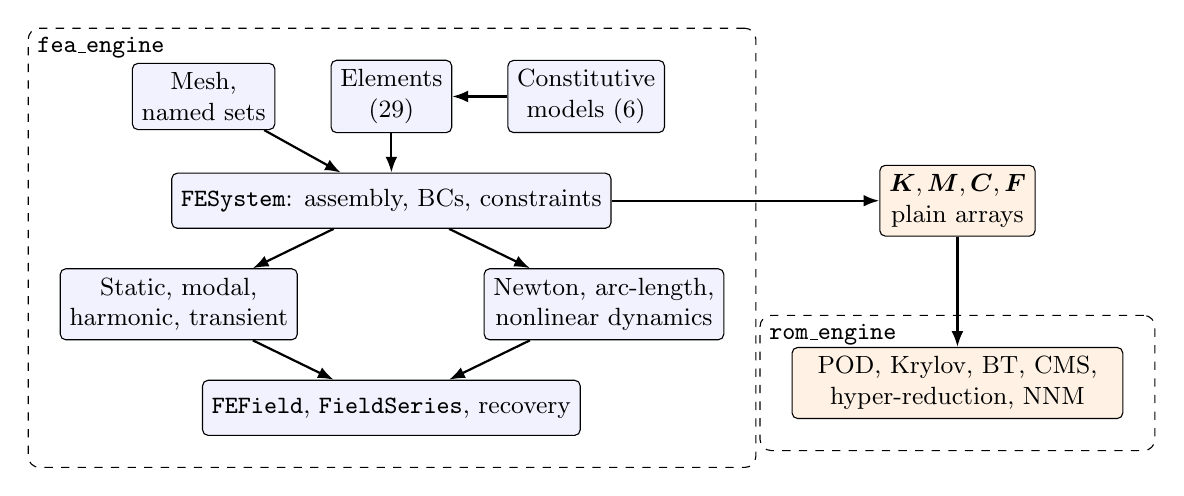
\begin{tikzpicture}[font=\small, node distance=5mm and 7mm,
  box/.style={draw, rounded corners=2pt, minimum height=7mm, align=center, fill=blue!5},
  grp/.style={draw, dashed, rounded corners=4pt, inner sep=4mm},
  arr/.style={-{Latex[length=2mm]}, thick}]
  \node[box] (mesh) {Mesh,\\named sets};
  \node[box, right=of mesh] (elem) {Elements\\(\nElements{})};
  \node[box, right=of elem] (mat) {Constitutive\\models (\nConstitutive{})};
  \node[box, below=of elem, minimum width=4.5cm] (sys) {\texttt{FESystem}: assembly, BCs, constraints};
  \node[box, below=of sys, xshift=-2.7cm] (ana) {Static, modal,\\harmonic, transient};
  \node[box, below=of sys, xshift=2.7cm] (nl) {Newton, arc-length,\\nonlinear dynamics};
  \node[box, below=of ana, xshift=2.7cm] (res) {\texttt{FEField}, \texttt{FieldSeries}, recovery};
  \node[box, right=34mm of sys, fill=orange!10] (arr) {$\K,\M,\C,\F$\\plain arrays};
  \node[box, below=14mm of arr, fill=orange!10, minimum width=4.2cm] (rom) {POD, Krylov, BT, CMS,\\hyper-reduction, NNM};
  \draw[arr] (mesh) -- (sys); \draw[arr] (elem) -- (sys); \draw[arr] (mat) -- (elem);
  \draw[arr] (sys) -- (ana); \draw[arr] (sys) -- (nl);
  \draw[arr] (ana) -- (res); \draw[arr] (nl) -- (res);
  \draw[arr] (sys) -- (arr); \draw[arr] (arr) -- (rom);
  \begin{scope}[on background layer]
    \node[grp, fit=(mesh)(elem)(mat)(sys)(ana)(nl)(res), label={[anchor=north west]north west:\fea}] {};
    \node[grp, fit=(rom), label={[anchor=north west]north west:\rom}, inner sep=4mm] {};
  \end{scope}
\end{tikzpicture}
\caption{Package structure. \rom{} sees only arrays; \texttt{FESystem} supplies them, but any other source can too.}
\label{fig:arch}
\end{figure}

\subsection{The \texttt{FESystem} pipeline}
A model is built in five steps: create a mesh with named node sets; choose an element and constitutive matrix;
assemble $\K$ and $\M$; apply constraints and loads; run an analysis. Elements and constitutive models are held in registries
(\nElements{} and \nConstitutive{} entries), so new ones can be added without changing the assembler.
Assembly follows the standard element-by-element scatter into sparse matrices \cite{zienkiewicz2013fem,bathe2014fep}, with a
vectorised path for elements whose kernels can be batched.

\subsection{Element interface}
Every element implements the same methods. With $\bm N$ the shape functions and $\bm B$ the strain--displacement matrix,
\begin{equation}
  \K_e=\int_{\Omega_e}\bm B^{\!\top}\bm D\,\bm B\,\mathrm{d}\Omega,\qquad
  \M_e=\int_{\Omega_e}\rho\,\bm N^{\!\top}\bm N\,\mathrm{d}\Omega,
  \label{eq:elem}
\end{equation}
evaluated by Gauss quadrature in the methods \texttt{shape\_and\_derivs}, \texttt{B\_matrix}, \texttt{stiffness} and \texttt{mass}.
Nonlinear analysis additionally uses \texttt{internal\_force} and \texttt{tangent\_stiffness}, which return $\bm f_{\mathrm{int}}(\vu_e)$
and $\partial\bm f_{\mathrm{int}}/\partial\vu_e$. Because all elements share this interface, the analysis layer does not branch on element type.

\subsection{Results and the safe interface}
Solver calls return result objects rather than bare vectors: \texttt{FEField} holds a nodal field with named components (for example
\texttt{"ux"}, \texttt{"uy"}) and can be queried by node set, and \texttt{FieldSeries} holds a sequence of such fields over time or load steps.
DOFs are addressed by name, quantities carry units where the API supports it, and the nonlinear solvers take a \texttt{NewtonOptions}
object instead of loose keyword arguments. The purpose is to turn common indexing errors (wrong DOF number, wrong component) into early
exceptions. Bare-array access remains available for performance-critical code.

\subsection{The FE/ROM boundary}
\rom{} classes such as \texttt{PodBasis} and \texttt{GalerkinROM} take $\K,\M,\F$ as SciPy sparse matrices or NumPy arrays.
A reduced system is returned as a \texttt{ReducedSystem}, which is itself a small set of matrices and can be solved, time-stepped,
or exported. Keeping the boundary at the array level means the same reduction code works on matrices from \fea{}, from a different
FE package, or from a lumped model.

\subsection{Optional PyTorch layer}
With PyTorch installed, linear systems can be solved on the CPU or GPU, and stress, strain and von~Mises fields can be recovered with
differentiable tensor operations. The solver selects a dense factorisation for fewer than 2000 free DOF and a Jacobi-preconditioned
conjugate gradient method otherwise, and raises an error if CG does not converge. All torch computations use double precision.
The recovery code is written once against a small operations shim that targets either NumPy or torch.
If PyTorch is absent, nothing else changes.

\subsection{Verification-first development}
Each element and solver is accompanied by tests that compare against analytical solutions or independent computations
(patch tests, beam theory, the elastica, and so on; \cref{sec:verif}). The suite runs \feaTests{} tests for \fea{} and \romTests{}
for \rom{}. We note that passing tests is evidence of correctness for the cases tested and not a proof for others; the limits are
listed in \cref{sec:limits}.

\subsection{A first example}
\Cref{lst:quick} builds a cantilever plate of \qsDof{} DOF (\qsFree{} free), solves it, constructs an \qsModes{}-mode POD basis from
snapshots of tip-traction loads, and solves the reduced model. The relative tip-deflection error between the full and reduced
models is \qsErr{} (the tip deflection is \qsTip{}~m). This error is small only because the test load lies in the span of
the snapshot loads; it is a consistency check of the pipeline and not a measure of ROM accuracy for unseen loads (see
\cref{sec:usage} for an out-of-sample test).

\lstinputlisting[caption={Quick-start: full model, POD basis and Galerkin reduction (\texttt{paper/listings/quickstart.py}).},label={lst:quick}]{listings/quickstart.py}


\section{Finite element formulation}\label{sec:fe}

This section states the continuum equations and the discrete operators that \fea{} assembles. The formulation is the standard displacement-based
one \cite{zienkiewicz2013fem,bathe2014fep}; we state it to fix notation and to make clear which parts of the code correspond to which equation.

\subsection{Weak form and discretisation}
For a body $\Omega$ with displacement field $\bm u(\bm x,t)$, density $\rho$, Cauchy stress $\bm\sigma$, body force $\bm b$ and traction $\bm t$ on $\Gamma_t$,
the principle of virtual work reads
\begin{equation}
  \int_\Omega \rho\,\delta\bm u\cdot\ddot{\bm u}\,\mathrm d\Omega
  +\int_\Omega \delta\bm\varepsilon:\bm\sigma\,\mathrm d\Omega
  =\int_\Omega\delta\bm u\cdot\bm b\,\mathrm d\Omega+\int_{\Gamma_t}\delta\bm u\cdot\bm t\,\mathrm d\Gamma
  \quad\forall\,\delta\bm u .
  \label{eq:weak}
\end{equation}
Approximating $\bm u\approx\bm N\vu$ with shape functions $\bm N$ and $\bm\varepsilon=\bm B\vu$, and taking linear elasticity $\bm\sigma=\bm D\bm\varepsilon$, gives the
semi-discrete equations
\begin{equation}
  \M\ddot{\vu}+\C\dot{\vu}+\K\vu=\F,
  \label{eq:sd}
\end{equation}
with $\K=\sum_e\K_e$ and $\M=\sum_e\M_e$ assembled from the element matrices \eqref{eq:elem}.
The damping matrix $\C$ is either Rayleigh damping $\C=\alpha\M+\beta\K$, with $(\alpha,\beta)$ calibrated to a target ratio $\zeta$ at two angular frequencies
$\omega_i,\omega_j$ by solving $\tfrac12\bigl(\alpha/\omega_k+\beta\omega_k\bigr)=\zeta$, $k\in\{i,j\}$ (\texttt{RayleighDamping.calibrate}),
or a modal damping ratio applied directly to decoupled modal equations (\texttt{ModalDamping}).
A lumped (diagonal) mass matrix is also available for explicit integration.

\subsection{Isoparametric elements and quadrature}
Two- and three-dimensional elements use isoparametric mapping: the geometry is interpolated with the same shape functions as the displacement,
$\bm x=\sum_a N_a(\bm\xi)\bm x_a$. With Jacobian $\bm J=\partial\bm x/\partial\bm\xi$, Cartesian derivatives are
$\partial N_a/\partial\bm x=\bm J^{-\top}\partial N_a/\partial\bm\xi$, and integrals over the element are evaluated by Gauss quadrature,
\begin{equation}
  \K_e\approx\sum_{p}w_p\,\bm B^{\!\top}(\bm\xi_p)\,\bm D\,\bm B(\bm\xi_p)\,\det\bm J(\bm\xi_p)\,t,
  \label{eq:gauss}
\end{equation}
where $t$ is the thickness for plane problems. Strains use engineering shear and the Voigt order $[xx,yy,xy]$ in 2-D and $[xx,yy,zz,xy,yz,xz]$ in 3-D.

\subsection{Element families}
\Cref{tab:elements} lists the element families. The registry holds \nElements{} entries; variants (for example selective-reduced and full integration of the same element) are
counted separately.

\begin{table}[t]
\centering\footnotesize
\caption{Element families in \fea{}. Class names are those in \texttt{fea\_engine.elements}.}
\label{tab:elements}
\begin{tabular}{>{\raggedright\arraybackslash}p{3.0cm}>{\raggedright\arraybackslash}p{5.2cm}>{\raggedright\arraybackslash}p{5.2cm}}
\toprule
Family & Classes & Formulation notes \\
\midrule
Trusses & \texttt{TrussTL2D}, \texttt{TrussPlastic2D} & total-Lagrangian, Green--Lagrange strain; 1-D elastoplastic variant \\
Beams, 2-D & \texttt{Beam2DEulerBernoulli}, \texttt{Beam2DCorotational}, \texttt{Beam2DReissner} & Hermite beam; corotational large rotation; shear-deformable planar beam \\
Beams, 3-D & \texttt{Beam3DEulerBernoulli}, \texttt{Beam3DCorotational} & per-element local axes; corotational variant \\
Plane stress/strain & \texttt{Tri3}, \texttt{Tri6}, \texttt{Quad4}, \texttt{Quad8}\texttt{PlaneStress} & isoparametric, Gauss quadrature \\
Solids & \texttt{Tet4}, \texttt{Tet10}, \texttt{Hex8}, \texttt{Hex20}\texttt{Solid3D}, \texttt{Hex8SolidBbar} & B-bar variant against volumetric locking \\
Plate & \texttt{Quad4MindlinPlate} & Mindlin--Reissner, selective reduced integration \\
Shells & \texttt{Shell4MITC}, \texttt{Shell4MITCCorotational}, \texttt{Shell4Director} & MITC4 assumed shear strain; corotational; degenerated-shell director kinematics (linear stiffness only, checked against MITC4) \\
Inelastic/hyperelastic & \texttt{Hex8PlasticJ2}, \texttt{Hex8PlasticJ2Kinematic}, \texttt{Quad4PlasticJ2PlaneStress}, \texttt{Tet4NeoHookean}, \texttt{Tet10SolidTL} & J2 plasticity; compressible Neo-Hookean; St~Venant--Kirchhoff-type total-Lagrangian 10-node tetrahedron \\
Contact & \texttt{GapContactPenalty}, \texttt{GapContactCurvedFriction}, \texttt{NodeToSegment\allowbreak Contact2D} (and friction variant) & penalty gap; node-to-segment with Coulomb friction \\
\bottomrule
\end{tabular}
\end{table}

\paragraph{Locking remedies.}
Low-order elements lock in the near-incompressible and thin limits. For the 8-node hexahedron, \texttt{Hex8SolidBbar} replaces the volumetric part of $\bm B$ by its element average,
\begin{equation}
  \bar{\bm B}_p=\bm B_p-\tfrac13\bm m\bm m^{\!\top}\bm B_p+\bar{\bm B}_{\mathrm{vol}},\qquad
  \bar{\bm B}_{\mathrm{vol}}=\frac{1}{V_e}\sum_q w_q\det\bm J_q\;\tfrac13\bm m\bm m^{\!\top}\bm B_q,
  \label{eq:bbar}
\end{equation}
with $\bm m=[1,1,1,0,0,0]^{\!\top}$ \cite{hughes1980bbar}. The 4-node Mindlin plate uses selective reduced integration of the shear term.
\texttt{Shell4MITC} follows the MITC4 element \cite{dvorkin1984}: the covariant transverse shear strains are sampled at the four edge mid-points and interpolated,
\begin{equation}
  \tilde e_{rt}=\tfrac12(1+s)\,e_{rt}^{(A)}+\tfrac12(1-s)\,e_{rt}^{(B)},\qquad
  \tilde e_{st}=\tfrac12(1+r)\,e_{st}^{(C)}+\tfrac12(1-r)\,e_{st}^{(D)},
  \label{eq:mitc}
\end{equation}
which removes shear locking in thin-shell bending. Membrane parts use the plane-stress $\bm B$ and bending parts the Mindlin curvature matrix. The element has a small penalty stiffness on the drilling rotation to
avoid singular matrices on flat patches. As in classic MITC4, membrane locking in coarse curved meshes is not addressed, and each element is a flat facet built from its own corner nodes.

\subsection{Assembly}
\Cref{alg:assembly} describes assembly. For a vectorised element the loop over $e$ is replaced by a batched kernel; otherwise the loop calls the element methods. Coordinates and
element constants may vary in space through coefficient fields (\cref{sec:recovery}).

\begin{algorithm}[t]
\caption{Global assembly of $\K$ (and, identically, $\M$)}\label{alg:assembly}
\begin{algorithmic}[1]
\Require mesh with connectivity $\{\mathcal I_e\}$, element formulation, constitutive matrix $\bm D$
\State $\K\gets\bm 0$ \Comment{sparse or dense, set at construction}
\For{each element $e$ of each block}
  \State $\bm x_e\gets$ nodal coordinates of $e$
  \State $\K_e\gets\sum_p w_p\bm B_p^{\!\top}\bm D\bm B_p\det\bm J_p\,t$ \Comment{element \texttt{stiffness}}
  \State $\mathcal G_e\gets$ global DOF indices from $\mathcal I_e$ and $n_{\mathrm{dof/node}}$
  \State $\K[\mathcal G_e,\mathcal G_e]\mathrel{+}=\K_e$
\EndFor
\State add spring and foundation terms (\cref{sec:constraints})
\end{algorithmic}
\end{algorithm}

\section{Boundary conditions and constraints}\label{sec:constraints}

\subsection{Prescribed DOFs}
Let the DOFs be partitioned into free ($f$) and prescribed ($c$) sets. With prescribed values $\vu_c$, the reduced static system is
\begin{equation}
  \K_{ff}\vu_f=\F_f-\K_{fc}\vu_c .
  \label{eq:dirichlet}
\end{equation}
\texttt{FESystem.form\_linear\_system} returns this system as a \texttt{ReducedSystem}, which stores $\K_{ff}$, the right-hand side, the index sets and the prescribed values,
and which can expand a reduced solution back to a full-length \texttt{FEField}. The same object is the interface used by iterative solvers and by the torch backend (\cref{sec:arch}).

\subsection{Springs and elastic foundations}
A grounded spring of stiffness $k$ on DOF $i$ adds $k$ to $K_{ii}$ (and $k\,u_{\mathrm{ref}}$ to $F_i$ if the spring rests at $u_{\mathrm{ref}}$). A Winkler foundation, or Robin boundary term,
$\bm t=k(\bm u-\bm u_{\mathrm{ref}})$ on a boundary $\Gamma_k$ contributes
\begin{equation}
  \K_k=\int_{\Gamma_k}k\,\bm N^{\!\top}\bm N\,\mathrm d\Gamma,\qquad
  \F_k=\int_{\Gamma_k}k\,\bm N^{\!\top}\bm u_{\mathrm{ref}}\,\mathrm d\Gamma,
  \label{eq:robin}
\end{equation}
evaluated over the element facets whose nodes all lie in the selected node set. The stiffness $k$ may be a function of position. These terms are stored and re-applied whenever
the stiffness matrix is re-assembled, so the order of calls does not matter.

\subsection{Linear multi-point constraints}
General constraints $\sum_i c_i u_i=g$, and equal-DOF ties between node pairs (including periodic boundaries via an offset vector), are eliminated exactly rather than imposed by penalty or multipliers.
Writing all constraints as $\bm C\vu_f=\bm g$, the code selects one dependent DOF per independent constraint by Gauss--Jordan elimination with full pivoting (largest coefficient) and expresses it through the others, which
yields
\begin{equation}
  \vu_f=\bm T\,\vu_r+\vu_p,\qquad
  \K_r=\bm T^{\!\top}\K_{ff}\bm T,\qquad
  \F_r=\bm T^{\!\top}\bigl(\F_f-\K_{ff}\vu_p\bigr),
  \label{eq:elim}
\end{equation}
where $\vu_r$ are the retained DOFs, $\bm T$ is sparse, and $\vu_p$ is a particular solution that carries the constraint values. If $\K_{ff}$ is symmetric positive definite, so is $\K_r$ whenever $\bm T$
has full column rank, which holds by construction. Chains of constraints and constraints that involve prescribed DOFs are handled in the same pass.
\Cref{alg:elim} summarises the procedure; modal analysis reduces the mass matrix with the same $\bm T$, $\M_r=\bm T^{\!\top}\M_{ff}\bm T$.

\begin{algorithm}[t]
\caption{Exact elimination of linear constraints}\label{alg:elim}
\begin{algorithmic}[1]
\Require $\K_{ff},\F_f$, constraint rows $(\bm c_k,g_k)$, prescribed values $\vu_c$
\State substitute prescribed DOFs into each constraint (moves terms to $g_k$)
\State \textbf{for} each constraint: pick the dependent DOF with the largest $|c|$ (full pivoting); express it through the remaining DOFs; redundant but consistent constraints are dropped, \textbf{raise an error} if equations conflict
\State build $\bm T$ (identity on retained DOFs, $-c_j/c_s$ on rows of dependent DOFs) and $\vu_p$
\State $\K_r\gets\bm T^{\!\top}\K_{ff}\bm T$;\quad $\F_r\gets\bm T^{\!\top}(\F_f-\K_{ff}\vu_p)$
\State solve $\K_r\vu_r=\F_r$;\quad $\vu_f\gets\bm T\vu_r+\vu_p$
\end{algorithmic}
\end{algorithm}

\paragraph{Current limits.}
Constraints are supported by the static and modal solvers; the transient, harmonic, buckling and nonlinear drivers raise \texttt{NotImplementedError} rather than ignore them.
Springs and foundations enter $\K$ and are therefore seen by all linear solvers, but the nonlinear drivers do not include them yet and also raise an error.
Reaction forces at constraints are not reported; \texttt{reactions} covers prescribed supports only.

\section{Linear analysis types}\label{sec:analysis}

\paragraph{Static.}
$\K_{ff}\vu_f=\F_f-\K_{fc}\vu_c$ \eqref{eq:dirichlet} is solved by sparse LU, dense Cholesky-type solves, or iterative methods (conjugate gradient and others, via \texttt{method=}).
For sparse systems the factorisation is available for reuse across right-hand sides, which the batched solver exploits (\cref{sec:perf}).

\paragraph{Modal.}
Natural frequencies and mode shapes solve the generalised eigenproblem
\begin{equation}
  \K_{ff}\bm\phi=\omega^2\M_{ff}\bm\phi,\qquad f=\omega/2\pi,
  \label{eq:eig}
\end{equation}
by a dense solver for dense systems and by shift-invert Lanczos at $\sigma=0$ for sparse ones, which targets the lowest modes. Eigenvectors are mass-normalised.

\paragraph{Linear buckling.}
For a reference state with geometric stiffness $\K_\sigma$ (built from a reference axial force, tension positive), the critical load factors $\lambda$ solve
$(\K+\lambda\K_\sigma)\bm\phi=\bm 0$, that is $\K\bm\phi=\lambda\,(-\K_\sigma)\bm\phi$, which has the same structure as \eqref{eq:eig}.
The result is meaningful only when $-\K_{\sigma,ff}$ is positive definite (a purely compressive reference state).

\paragraph{Harmonic response and random vibration.}
At a driving frequency $\Omega$ the code solves $(\K-\Omega^2\M+\mathrm i\Omega\C)\bm U=\bm F_0$ directly for the complex amplitude; at $\Omega=0$ this reduces to the static solve.
Random vibration is built on the harmonic sweep: with the transfer function $H(f)$ from a unit load pattern to an output DOF, the output power spectral density is
$S_{\mathrm{out}}(f)=|H(f)|^2S_{\mathrm{in}}(f)$ and the RMS response is $\sigma=\bigl(\int S_{\mathrm{out}}\,\mathrm df\bigr)^{1/2}$, integrated by the trapezoidal rule.

\paragraph{Transient.}
Implicit integration uses the Newmark-$\beta$ family \cite{newmark1959}. With displacement predictors, the effective stiffness for \eqref{eq:sd} is
\begin{equation}
  \K_{\mathrm{eff}}=\K+a_0\M+a_1\C,\qquad a_0=\frac{1}{\beta\Delta t^2},\quad a_1=\frac{\gamma}{\beta\Delta t},
  \label{eq:keff}
\end{equation}
which for the default $\beta=\tfrac14,\gamma=\tfrac12$ (average acceleration) is unconditionally stable for linear systems. For a linear system $\K_{\mathrm{eff}}$ is constant, and
it is factorised once before the time loop. Explicit integration is the central-difference recursion on a lumped mass matrix, stable for $\Delta t\le2/\omega_{\max}$; \texttt{critical\_timestep}
computes $\omega_{\max}$ from the full spectrum, and a local estimate from element wave speeds is provided for large systems. Modal superposition integrates $n$ decoupled single-DOF equations with a given damping ratio per mode and
reconstructs $\vu(t)=\bm\Phi\bm q(t)$.

\section{Nonlinear analysis}\label{sec:nonlinear}

\subsection{Nonlinear equilibrium and Newton's method}
For a geometrically or materially nonlinear structure the discrete equilibrium is
$\bm r(\vu,\lambda)=\lambda\,\fext^{\mathrm{ref}}-\fint(\vu)=\bm 0$ on the free DOFs, with load factor $\lambda$. Each element supplies $\fint$ and its consistent tangent
$\KT=\partial\fint/\partial\vu$; the base element class falls back to $\fint=\K_e\vu_e$ and $\KT=\K_e$, so linear elements run through the same drivers (and converge in one iteration).
In the load-controlled driver, $\lambda$ increases over a prescribed array of load factors (a ramp by default, or any history including unloading). \Cref{alg:newton} gives one load step.

\begin{algorithm}[t]
\caption{One load step of incremental Newton--Raphson}\label{alg:newton}
\begin{algorithmic}[1]
\Require converged $\vu_n$, new load factor $\lambda$, tolerance $\epsilon$
\State $\vu\gets\vu_n$;\quad $\mathrm{ref}\gets\max(\|\lambda(\fext^{\mathrm{ref}})_f\|,10^{-30})$
\For{$k=1,\dots,k_{\max}$}
  \State $\bm r\gets\lambda(\fext^{\mathrm{ref}})_f-\fint(\vu)_f$
  \State \textbf{if} $\|\bm r\|<\epsilon\,\mathrm{ref}$ \textbf{or} $\|\bm r\|<\epsilon$ (plus optional step-size and energy tests) \textbf{then stop}
  \State solve $\KT(\vu)_{ff}\,\delta\vu=\bm r$
  \State (optional) Armijo backtracking on $\delta\vu$
  \State $\vu\gets\vu+\delta\vu$;\quad update iteration-level internal state
\EndFor
\State commit element state variables at $\vu$ (history for plasticity)
\end{algorithmic}
\end{algorithm}

The step-size and energy tests and the Armijo line search are off by default and are configured through the shared \texttt{NewtonOptions} object. Displacement control prescribes one DOF
and records the reaction needed to hold it, which allows following paths with a limit load.

\subsection{Path following}
Near limit points the load-controlled iteration fails. \texttt{solve\_nonlinear\_arc\_length} implements the cylindrical arc-length method of Crisfield \cite{crisfield1981}
(see also \cite{riks1979}), where the load factor is an unknown and each step satisfies
\begin{equation}
  \bm r(\vu,\lambda)=\bm 0,\qquad \|\Delta\vu\|^2=\Delta\ell^2 ,
  \label{eq:arc}
\end{equation}
with $\Delta\vu$ the step increment over the free DOFs. Each iteration writes $\delta\vu=\delta\vu_r+\delta\lambda\,\delta\vu_F$ with $\delta\vu_F=\KT^{-1}\fext^{\mathrm{ref}}$,
which turns the constraint into a quadratic in $\delta\lambda$; of the two roots, the one whose increment has the larger inner product with the increment accumulated so far in the step is taken, so the path
keeps moving forward. The arc-length $\Delta\ell$ is fixed by the user and is not adapted.

\texttt{solve\_nonlinear\_koiter\_newton} replaces the linear tangent predictor with a cubic one from an asymptotic expansion of the equilibrium path. Writing $\bm w=\vu-\vu_n$ and keeping terms up to third order,
\begin{equation}
  \bm L(\bm w)+\bm Q(\bm w,\bm w)+\bm C(\bm w,\bm w,\bm w)=\Delta\lambda\,\fext^{\mathrm{ref}},\qquad \bm L=\KT(\vu_n),
  \label{eq:koiter}
\end{equation}
with $\bm Q,\bm C$ the quadratic and cubic terms of the Taylor series of $\fint$; $\bm w$ and $\Delta\lambda$ are expanded in a scalar perturbation parameter, and the resulting linear problems
are solved with the factorised tangent. The coefficients of $\bm Q$ and $\bm C$ are extracted along the perturbation direction by central finite differences of $\fint$, with a probe length proportional to the
step's displacement scale, so elements need only provide $\fint$. The implementation follows the Koiter--Newton method of Liang et al.\ \cite{liang2014koiternewton} for a single perturbation direction; a second
driver adds a second direction built from a near-critical tangent mode when one is detected (mode interaction). Newton globalisation options (step-size test, line search) are not available in the Koiter--Newton correctors.

\subsection{Elements for large rotations and strains}
\paragraph{Trusses and beams.}
\texttt{TrussTL2D} uses the Green--Lagrange strain $E=(l^2-L_0^2)/(2L_0^2)$ with current length $l$ and St~Venant--Kirchhoff stress $S=EE$ (modulus $E$), giving
$\bm f=(SA/L_0)\,\bm d$ with $\bm d$ the current relative position; the tangent is the sum of a material and a geometric part.
\texttt{Beam2DCorotational} and \texttt{Beam3DCorotational} follow the corotational idea of separating rigid-body motion from small local deformation \cite{crisfield1990corot}.
\texttt{Beam2DReissner} is a two-node shear-deformable planar beam with exact strain measures in the Simo--Reissner sense \cite{simo1985beam}, with axial, shear and curvature strains $(\varepsilon,\gamma,\kappa)$
computed from the current configuration, and a shear correction factor passed in the material tuple.

\paragraph{Plasticity.}
For small-strain J2 plasticity with linear isotropic hardening (yield stress $\sigma_y$, hardening modulus $H$), the update is the elastic-predictor, radial-return algorithm \cite{simo1985tangent,simo1998inelasticity}.
Split the trial stress into volumetric and deviatoric parts, $\bm s^{\mathrm{tr}}=2\mu\,\mathrm{dev}(\bm\varepsilon-\bm\varepsilon^p_n)$. The yield function is
$f=\|\bm s^{\mathrm{tr}}\|-\sqrt{\tfrac23}(\sigma_y+H\alpha_n)$. If $f\le0$ the step is elastic. Otherwise
\begin{equation}
  \Delta\gamma=\frac{f}{2\mu+\tfrac23H},\qquad
  \bm s=\bm s^{\mathrm{tr}}-2\mu\,\Delta\gamma\,\bm n,\quad \bm n=\frac{\bm s^{\mathrm{tr}}}{\|\bm s^{\mathrm{tr}}\|},\qquad
  \alpha=\alpha_n+\sqrt{\tfrac23}\,\Delta\gamma,
  \label{eq:j2}
\end{equation}
a closed-form radial rescaling in deviatoric space with no local iteration. The algorithmic (consistent) tangent is obtained by differentiating the discrete update \cite{simo1985tangent}. The plane-stress variant
needs a local iteration and is a separate routine, and a kinematic-hardening version exists for the 3-D element.
State variables are evaluated afresh at every Newton iteration and committed only after a converged step.
\texttt{Tet4NeoHookean} uses the compressible Neo-Hookean energy $W=\tfrac{\mu}{2}(\bar I_1-3)+\tfrac{\kappa}{2}(J-1)^2$ with $\bar I_1=J^{-2/3}\operatorname{tr}\bm C$, $J=\det\bm F$,
$\bm C=\bm F^{\!\top}\bm F$, whose second Piola--Kirchhoff stress is
$\bm S=\mu J^{-2/3}\bigl(\bm I-\tfrac13\operatorname{tr}(\bm C)\,\bm C^{-1}\bigr)+\kappa J(J-1)\bm C^{-1}$. It does not treat the incompressible limit, which requires a mixed formulation.

\subsection{Nonlinear dynamics}
Implicit nonlinear dynamics applies Newmark's method with Newton iteration in each step. With the Newmark relations for acceleration and velocity affine in the trial displacement $\bm d$,
the residual and its exact derivative are
\begin{equation}
  \bm R(\bm d)=\M\bm a(\bm d)+\C\bm v(\bm d)+\fint(\bm d)-\fext(t+\Delta t),\qquad
  \K_{\mathrm{eff}}(\bm d)=\KT(\bm d)+a_0\M+a_1\C ,
  \label{eq:nl-newmark}
\end{equation}
so the effective matrix is re-factorised every iteration. For a linear element this reduces to the linear Newmark solver of \cref{sec:analysis} and Newton converges in one step.
The explicit nonlinear integrator uses central differences on a lumped mass, so no Newton loop is needed and each step costs one internal-force evaluation.

\subsection{Contact}
\Cref{tab:contact} lists the contact formulations. Penalty contact is a unilateral spring on the penetration $\delta=\bm n\cdot\bm u-g_0$: $\bm f=k_p\max(\delta,0)\,\bm n$ with tangent $k_p\bm n\bm n^{\!\top}$ while active
\cite{wriggers2006contact}. The Lagrange multiplier version enforces $\delta=0$ exactly through one extra unknown $\lambda$ by solving the bordered Newton system
\begin{equation}
  \begin{bmatrix}\KT&\bm n\\ \bm n^{\!\top}&0\end{bmatrix}
  \begin{bmatrix}\delta\vu\\ \delta\lambda\end{bmatrix}=
  \begin{bmatrix}\fext-\fint-\lambda\bm n\\ g_0-\bm n\cdot\vu\end{bmatrix},
  \label{eq:kkt}
\end{equation}
after first checking whether the unconstrained step penetrates (active-set strategy). The augmented-Lagrangian version replaces the multiplier solve by Uzawa updates $\bar\lambda\leftarrow\max(\bar\lambda+k_p\delta,0)$
on top of a penalty Newton solve, driving the penetration to zero for any $k_p$.

\begin{table}[t]
\centering\footnotesize
\caption{Contact formulations and their scope.}\label{tab:contact}
\begin{tabular}{>{\raggedright\arraybackslash}p{4.2cm}>{\raggedright\arraybackslash}p{4.3cm}>{\raggedright\arraybackslash}p{4.5cm}}
\toprule
Formulation & Implementation & Scope \\
\midrule
Penalty gap & \texttt{GapContactPenalty} (fixed normal), \texttt{GapContactCurvedFriction} (curved obstacle, Coulomb friction) & analytic rigid obstacle \\
Node-to-segment & \texttt{NodeToSegmentContact2D}, \texttt{...Friction} & 2-D, both bodies deformable; broad-phase helper \texttt{find\_contact\_pairs\_2d} \\
Lagrange multiplier & \texttt{solve\_contact\_\allowbreak lagrange\_\allowbreak static} & one contact node, monotonic engagement \\
Augmented Lagrangian & \texttt{solve\_contact\_\allowbreak augmented\_\allowbreak lagrange\_\allowbreak static} & same scope as Lagrange \\
\bottomrule
\end{tabular}
\end{table}

The multiplier and augmented-Lagrangian solvers handle a single contact node. General multi-point contact uses the penalty elements.

\section{Derived results and spatially varying coefficients}\label{sec:recovery}

\subsection{Stress and strain recovery}
Displacements are the primary unknowns; strains and stresses are computed at integration points, $\bm\varepsilon_p=\bm B_p\vu_e$ and $\bm\sigma_p=\bm D(\bm x_p)\bm\varepsilon_p$, and then moved to the nodes.
\fea{} uses a lumped $L^2$ projection with the linear (corner-node) shape functions $N_a$:
\begin{equation}
  \bm\sigma_a=\frac{\sum_{e\ni a}\sum_p N_a(\bm\xi_p)\,\bm\sigma_p\,\det\bm J_p\,w_p}{\sum_{e\ni a}\sum_p N_a(\bm\xi_p)\,\det\bm J_p\,w_p}.
  \label{eq:l2}
\end{equation}
The weights are non-negative, so the nodal value is a weighted mean of integration-point values and cannot overshoot them; for constant-strain triangles and tetrahedra it reduces to the usual volume-weighted average.
Mid-side nodes of quadratic elements are interpolated from the corner values, because projecting with a quadratic shape function (which integrates to zero or less at a corner) is ill-posed.
This is simple and robust but is not a superconvergent recovery such as \cite{zienkiewicz1992spr}, and values on a boundary are smoothed estimates (compare \cite{hinton1974smoothing}, which also discusses smoothing of discontinuous finite element functions).
The von~Mises equivalent stress is computed from the nodal components, for plane stress, plane strain (with Poisson's ratio) or 3-D,
$\sigma_{\mathrm{vM}}=\sqrt{\tfrac32\,\bm s\!:\!\bm s}$ with $\bm s$ the deviatoric stress. Reactions at supports are $\bm R_c=\K_{cf}\vu_f+\K_{cc}\vu_c-\F_c$.

Supported elements are the plane-stress triangles and quadrilaterals (Tri3, Tri6, Quad4, Quad8) and the 3-D solids (Tet4, Tet10, Hex8, Hex20) with full integration. Results are \texttt{FEField} objects, so they
can be queried by node set and exported with the same interface as displacements.

\subsection{Batched and differentiable recovery}
The recovery loop over elements is expressed once as array operations on arrays of shape (elements, integration points, \dots), through a thin operations shim that dispatches to NumPy or PyTorch. The NumPy path
replaces the per-element Python loop; the torch path additionally returns tensors that carry gradients with respect to the displacement vector, so quantities such as a maximum von~Mises stress can be differentiated.
Coefficient fields that vary by position use the element loop; the torch path does not support coefficients. Measured speed-ups of the batched path are reported in \cref{sec:perf}.

\subsection{Spatially varying coefficients}
Material parameters, foundation stiffness and similar coefficients can be given as functions of the physical coordinate $\bm x$, evaluated at integration points; $\bm D(\bm x)$ in \eqref{eq:gauss} then varies within the element.
Recovery uses the same coefficient, so stress is consistent with the stiffness that produced the displacement.

\section{Reduced-order modelling in \texorpdfstring{\rom{}}{rom\_engine}}\label{sec:rom}

This section states the methods in \rom{}. All of them are established; the contribution here is a uniform array-level implementation and the way the pieces compose. We write $n$ for the full dimension and $r\ll n$ for the reduced one, and
assume $\K,\M$ are symmetric with $\K$ positive definite on the free DOFs. The general setting and its literature are in \cite{benner2015survey,hesthaven2016rb,antoulas2005}.

\subsection{Projection-based reduction}\label{sec:rom:proj}
\paragraph{Bases.}
A reduced basis $\bm V\in\mathbb R^{n\times r}$ gives the approximation $\vu\approx\bm V\bm q$. For snapshots $\bm X=[\vu^{(1)},\dots,\vu^{(m)}]$ the proper orthogonal decomposition (POD) is the
truncated singular value decomposition $\bm X\approx\bm U_r\bm\Sigma_r\bm W_r^{\!\top}$, which is the best rank-$r$ approximation in the Frobenius norm \cite{berkooz1993pod}.
For structural models the Euclidean norm mixes translations and rotations, so \texttt{PodBasis.fit(\dots, M=M)} uses the mass inner product: with the Cholesky factor $\M=\bm L\bm L^{\!\top}$,
\begin{equation}
  \tilde{\bm X}=\bm L^{\!\top}\bm X=\tilde{\bm U}\bm\Sigma\bm W^{\!\top},\qquad \bm V=\bm L^{-\top}\tilde{\bm U}_r,\qquad \bm V^{\!\top}\M\bm V=\bm I_r .
  \label{eq:pod}
\end{equation}
The rank is set by a count or by an energy fraction $\sum_{i\le r}\sigma_i^2/\sum_i\sigma_i^2$. Mode shapes from \texttt{solve\_modal} are also valid bases, and a multi-field variant fits separate fields with a block-diagonal weight.

\paragraph{Galerkin projection.}
Requiring the residual to be orthogonal to the basis, $\bm V^{\!\top}(\K\bm V\bm q-\F)=\bm 0$, gives the reduced system
\begin{equation}
  \K_r\bm q=\F_r,\qquad \K_r=\bm V^{\!\top}\K\bm V,\ \ \M_r=\bm V^{\!\top}\M\bm V,\ \ \F_r=\bm V^{\!\top}\F .
  \label{eq:galerkin}
\end{equation}
For symmetric positive definite $\K$ this is the best approximation in $\operatorname{range}(\bm V)$ in the energy norm, the same variational argument that makes the finite element method a Galerkin method. \texttt{GalerkinROM} also solves the reduced
eigenproblem $\K_r\bm\phi=\omega^2\M_r\bm\phi$ and expands results to full coordinates by $\vu=\bm V\bm q$.

\paragraph{Static completion of truncated modes.}
A truncated modal basis omits the static contribution of the discarded modes. Two closed-form remedies (mode acceleration and modal truncation augmentation) \cite{besselink2013comparison} are provided. The static correction for a load $\F$ is
\begin{equation}
  \bm q_{\mathrm{cor}}=\K^{-1}\F-\bm V\bigl(\bm V^{\!\top}\K\bm V\bigr)^{-1}\bm V^{\!\top}\F,
  \label{eq:modeacc}
\end{equation}
which needs one full static solve; it can be added after the fact or appended to the basis after $\M$-orthogonalisation against $\bm V$. An error is raised if the correction already lies in $\operatorname{range}(\bm V)$.

\subsection{Parametric problems and certified error}\label{sec:rom:param}
\paragraph{Affine decomposition and the offline--online split.}
If $\K(\bm\mu)=\sum_{q=1}^{Q}\theta_q(\bm\mu)\K_q$ with fixed matrices $\K_q$ (for example one per material region, each assembled with unit modulus), the reduced matrices are
$\K_r(\bm\mu)=\sum_q\theta_q(\bm\mu)\,\bm V^{\!\top}\K_q\bm V$; the projections $\bm V^{\!\top}\K_q\bm V$ are computed once, and each query costs $O(Qr^2+r^3)$, independent of $n$. The decomposition is exact when the physics is affine in the parameters, which holds for linear elasticity in Young's modulus.
\Cref{alg:offline} shows the split.

\begin{algorithm}[t]
\caption{Offline--online reduced-basis solve with affine parameters}\label{alg:offline}
\begin{algorithmic}[1]
\Require snapshots $\bm X$, affine terms $\{\K_q\}$, load $\F$
\State \textbf{Offline:} $\bm V\gets$ POD$(\bm X)$ \eqref{eq:pod}; $\K_q^r\gets\bm V^{\!\top}\K_q\bm V$ for all $q$; $\F_r\gets\bm V^{\!\top}\F$
\State \textbf{Online, for each $\bm\mu$:}
\State \quad $\K_r\gets\sum_q\theta_q(\bm\mu)\K_q^r$; \ solve $\K_r\bm q=\F_r$; \ $\vu\gets\bm V\bm q$ (only if the full field is needed)
\end{algorithmic}
\end{algorithm}

\paragraph{Frequency domain.}
Harmonic response has $\bm A(\omega)\bm X=\F$ with $\bm A(\omega)=-\omega^2\M+\mathrm i\omega\C+\K$, which is affine in $\{\M,\C,\K\}$ with $\bm\theta(\omega)=[-\omega^2,\ \mathrm i\omega,\ 1]$. \texttt{FrequencyROM} is this decomposition composed with Galerkin projection, so a sweep of thousands of frequencies solves $r\times r$ systems.
A basis can be trained on POD of response snapshots at chosen frequencies.

\paragraph{Weak greedy selection.}
Instead of a uniform frequency grid, \cref{alg:greedy} picks training frequencies where the current basis is weakest, which concentrates full-order solves near resonances. The indicator is the difference between the current reduced response and that of the previous (smaller) model evaluated at every untried frequency, the hierarchical error indicator of the weak-greedy construction \cite{hesthaven2016rb}.

\begin{algorithm}[t]
\caption{Weak-greedy frequency basis}\label{alg:greedy}
\begin{algorithmic}[1]
\Require candidate frequencies $\Omega$, seed size $n_0$, tolerance $\epsilon$, maximum size $r_{\max}$
\State choose $n_0$ seed frequencies; solve full-order at each; build $\bm V$ and the reduced model $\mathcal R_k$
\For{$k=1,2,\dots$ until $r\ge r_{\max}$}
  \State for each untried $\omega\in\Omega$: $\eta(\omega)\gets\|\mathcal R_k(\omega)-\mathcal R_{k-1}(\omega)\|$ \Comment{reduced queries only}
  \State $\omega^\ast\gets\arg\max\eta$;\ \textbf{stop if} $\eta(\omega^\ast)<\epsilon$
  \State solve full-order at $\omega^\ast$; rebuild $\bm V$ and $\mathcal R_{k+1}$
\EndFor
\end{algorithmic}
\end{algorithm}

\paragraph{A posteriori bound.}
For any reduced solution $\bm x_r$, the residual $\bm\rho=\F-\bm A(\omega)\bm x_r$ gives
$\|\bm x-\bm x_r\|\le\|\bm\rho\|/\sigma_{\min}(\bm A(\omega))$,
so a rigorous error bound needs a lower bound on the smallest singular value. \rom{} provides two. The first uses Weyl's inequality $|\sigma_{\min}(\bm A)-\sigma_{\min}(\bm B)|\le\|\bm A-\bm B\|_2$ around reference frequencies
$\omega_j$, applied term by term to the affine form $\bm A=\sum_q\theta_q\bm A_q$, which gives $\sigma_{\min}(\bm A(\omega))\ge\max\Bigl(0,\max_j\bigl[\sigma_{\min}(\bm A(\omega_j))-\sum_q|\theta_q(\omega)-\theta_q(\omega_j)|\,\|\bm A_q\|_2\bigr]\Bigr)$ with reference points chosen greedily. The second is the successive constraint method (SCM) of Huynh et al.\ \cite{huynh2007scm} through a small linear program, applied to the real symmetric positive semi-definite matrix
$\bm A^{\!\mathsf H}\bm A$ so that complex, non-Hermitian operators are covered. The sharper natural-norm variant for non-coercive operators is not implemented. Away from the reference frequencies the bound can fall to zero, which is valid but uninformative; adding references tightens it and never invalidates it.

\subsection{System-theoretic reduction}\label{sec:rom:sys}
With input matrix $\bm B$ (load pattern) and output matrix $\bm C_{\mathrm o}$ (selected DOFs), the second-order system is cast into first-order form with state $[\bm q;\dot{\bm q}]$, giving $\bm E\dot{\bm x}=\bm A\bm x+\bm Bu$, $y=\bm C_{\mathrm o}\bm x$ in two algebraically equivalent forms.
Four families follow the classification of Besselink et al.\ \cite{besselink2013comparison}.

\paragraph{Krylov moment matching.}
Expanding the transfer function $H(s)=\bm C_{\mathrm o}(s\bm E-\bm A)^{-1}\bm B$ about $s_0$, a basis of the Krylov subspace $\mathcal K_k\bigl((\bm A-s_0\bm E)^{-1}\bm E,(\bm A-s_0\bm E)^{-1}\bm B\bigr)$ built by block Arnoldi gives a reduced model that matches the first moments at $s_0$. The approximation is local: accurate near $s_0$ and degrading away from it. A two-sided (Petrov--Galerkin) option builds a second basis from the dual system.
SOAR (second-order Arnoldi) \cite{bai2005soar} matches the same moments from the second-order pencil $H(s)=\bm C_{\mathrm o}(s^2\M+s\C+\K)^{-1}\bm B$ without forming the first-order system, using the two-term recurrence $\bm\Phi_j=\bm A_1\bm\Phi_{j-1}+\bm A_2\bm\Phi_{j-2}$ with
$\bm A_1=-\bm K_0^{-1}(\C+2s_0\M)$, $\bm A_2=-\bm K_0^{-1}\M$, $\bm K_0=\K+s_0\C+s_0^2\M$.

\paragraph{Balanced truncation.}
Balanced truncation \cite{moore1981} solves the two Lyapunov equations
\begin{equation}
  \bm A\bm P+\bm P\bm A^{\!\top}+\bm B\bm B^{\!\top}=\bm 0,\qquad
  \bm A^{\!\top}\bm Q+\bm Q\bm A+\bm C_{\mathrm o}^{\!\top}\bm C_{\mathrm o}=\bm 0,
  \label{eq:lyap}
\end{equation}
balances them to equal diagonal Gramians whose entries are the Hankel singular values $\sigma_1\ge\sigma_2\ge\cdots$, and keeps the $r$ states with the largest $\sigma_i$. It preserves stability and satisfies the a priori bound
$\|G-G_r\|_{\mathcal H_\infty}\le2\sum_{i>r}\sigma_i$ \cite{enns1984,glover1984}; the code returns this bound with the model. Because it uses the ports, balanced truncation is accurate over the whole frequency axis rather than near one point.
Related variants in the package are singular perturbation approximation \cite{liu1989spa}, which preserves the DC gain, frequency-weighted balanced truncation with low-pass and band-pass weights, and optimal Hankel-norm approximation, whose realisation \cite{glover1984} attains $\|G-G_r\|_{\mathrm H}=\sigma_{r+1}$ exactly but is implemented for single-input single-output systems only.
A passivity diagnostic is also provided: for a collocated force input and velocity output, the energy balance $\dot E=-\dot{\bm q}^{\!\top}\C\dot{\bm q}+u\,y\le u\,y$ holds when $\C$ is positive semi-definite, so passivity can be certified in closed form for the full model and checked numerically for the reduced one.

\paragraph{Data-driven identification.}
\texttt{LoewnerROM} identifies natural frequencies, damping ratios and mode shapes from sampled frequency responses alone, using the Loewner pencil built from two disjoint frequency sets \cite{mayo2007loewner}. It never receives $\K$, $\M$ or $\C$, so it applies to measured data.

\subsection{Nonlinear reduction}\label{sec:rom:nl}
\paragraph{Intrusive nonlinear Galerkin.}
Projecting $\M\ddot{\vu}+\C\dot{\vu}+\fint(\vu)=\fext(t)$ gives
$\M_r\ddot{\bm q}+\C_r\dot{\bm q}+\bm V^{\!\top}\fint(\bm V\bm q)=\bm V^{\!\top}\fext(t)$
with full (not diagonal, not mass-normalised) reduced matrices, as in the POD--Galerkin reduction of a planar nonlinear rod \cite{georgiou2005}. The reduced tangent $\K_r$ is computed once from the full tangent at $\vu=\bm 0$,
and the nonlinear part is $\bm f_{\mathrm{nl}}(\bm q)=\bm V^{\!\top}\fint(\bm V\bm q)-\K_r\bm q$. Integration is by Newton--Newmark, Runge--Kutta or a generic ODE solver. The cost per step is still proportional to the full model because $\fint(\bm V\bm q)$ is evaluated at all elements, which motivates hyper-reduction.

\paragraph{Hyper-reduction.}
Energy-conserving sampling and weighting (ECSW) \cite{farhat2015ecsw} approximates the reduced force by a weighted sum over a small element subset $\mathcal E$,
\begin{equation}
  \bm f_r(\bm q)=\sum_{e=1}^{n_e}\bm V_e^{\!\top}\bm f_e(\bm V_e\bm q)\ \approx\ \sum_{e\in\mathcal E}w_e\,\bm V_e^{\!\top}\bm f_e(\bm V_e\bm q),\quad w_e\ge0 ,
  \label{eq:ecsw}
\end{equation}
where $\bm V_e$ are the rows of $\bm V$ for element $e$. The weights solve a non-negative least-squares problem built from training states (\cref{alg:ecsw}) with the active-set solver of Lawson and Hanson \cite{lawson1995lsq}, stopped when the relative residual is below a tolerance, which keeps $\mathcal E$ small.
Positive weights over real element contributions preserve the symmetry and positive definiteness of the reduced tangent.

\begin{algorithm}[t]
\caption{ECSW weight training}\label{alg:ecsw}
\begin{algorithmic}[1]
\Require basis $\bm V$, training states $\{\vu^{(k)}\}_{k=1}^{m}$, element force callbacks $\bm f_e$, tolerance $\epsilon$
\State for each $k$ and $e$: $\bm G_{ke}\gets\bm V_e^{\!\top}\bm f_e(\vu^{(k)}_e)$ (element force at the snapshot's own element DOFs), stack over $k$ into column $e$ of $\bm G$
\State $\bm b\gets\sum_e\bm G_{:e}$ \Comment{exact reduced force}
\State solve $\min_{\bm w\ge0}\|\bm G\bm w-\bm b\|$ by Lawson--Hanson NNLS, stopping when $\|\bm G\bm w-\bm b\|\le\epsilon\|\bm b\|$
\State $\mathcal E\gets\{e:w_e>0\}$
\end{algorithmic}
\end{algorithm}

Discrete empirical interpolation (DEIM) \cite{chaturantabut2010deim} instead approximates the force vector from its values at $m$ interpolation DOFs, $\bm f\approx\bm U(\bm P^{\!\top}\bm U)^{-1}\bm P^{\!\top}\bm f$, where $\bm U$ is a POD basis of force snapshots and $\bm P$ selects the DOFs;
QDEIM selects them by column-pivoted QR of $\bm U^{\!\top}$ \cite{drmac2016qdeim}. Gappy reconstruction is the same interpolation applied to a field. ECSW needs per-element force callbacks; DEIM does not.

\paragraph{Surrogate (implicit-condensation) ROMs.}
In a hybrid reduced model the linear part is intrusive and only the nonlinear modal force is fit from data. In mass-normalised modal coordinates
\begin{equation}
  \ddot{\bm q}+\C_r\dot{\bm q}+\bm\Lambda\bm q+\bm F_{\mathrm{nl}}(\cdot)=\bm F_{\mathrm{ext}}(t),
  \label{eq:hybrid}
\end{equation}
where $\bm\Lambda=\operatorname{diag}(\omega_i^2)$. Two regressions of $\bm F_{\mathrm{nl}}$ are provided, both following published methods:
(i) the implicit condensation and expansion (ICE) method of Hollkamp and Gordon \cite{hollkamp2008ice}, in which $\bm F_{\mathrm{nl}}$ is a quadratic-plus-cubic polynomial in the modal displacements, fit by least squares to full-order solutions under sampled static loads (reviewed in \cite{mignolet2013review}); and
(ii) the multi-fidelity-surrogate method (MFS-NLROM) of He et al.\ \cite{he2023mfsnlrom}, where $\bm F_{\mathrm{nl}}$ is a radial-basis-function interpolant of the \emph{linear} modal displacement,
\begin{equation}
  \bm F_{\mathrm{nl}}(\bm q_l)=\sum_{j=1}^{N}\bm w_j\,\varphi\bigl(\|\bm q_l-\bm q_{l,j}\|\bigr),\qquad \bm W=(\bm\Psi+\varepsilon\,\tfrac{\operatorname{tr}\bm\Psi}{N}\bm I)^{-1}\bm F_{\mathrm{train}},
  \label{eq:rbf}
\end{equation}
with kernel $\varphi$ (multiquadric by default) and a small ridge $\varepsilon$ for conditioning. Because the argument is the linear displacement, evaluating \eqref{eq:rbf} needs no Newton iteration; the polynomial version, which is a function of the nonlinear coordinates, does for static loads. Training data come from applied-load or enforced-displacement strategies. A small neural network can replace the RBF interpolant through the same protocol.
For dynamics, the reduced equations are integrated by Newmark with the nonlinear force lagged by one step and corrected by fixed-point iteration with four iterations (default), by a sign-deviation predictor following He et al., or by Newton. The fixed-point default was
adopted because one-shot lagging was found to accumulate error and diverge on the flat-beam benchmark. Membrane expansion, which adds the in-plane response that flat-beam bending modes lack, follows the ICE paper.

\paragraph{Nonlinear normal modes.}
For the undamped autonomous system, periodic solutions are written as truncated Fourier series $\bm q(t)=\bm Z_0+\sum_{k=1}^{H}[\bm a_k\cos k\omega t+\bm b_k\sin k\omega t]$, and the harmonic-balance equations
\begin{equation}
  \bm h(\bm Z,\omega)=\bm A(\omega)\bm Z+\bm F_{\mathrm{nl}}^{\mathrm{harm}}(\bm Z)=\bm 0
  \label{eq:hbm}
\end{equation}
are solved with the nonlinear force evaluated by alternating frequency--time (AFT) transforms, as in the NNM literature \cite{kerschen2009nnm}. The backbone, frequency against amplitude of a chosen mode, is traced either by natural-parameter continuation in the amplitude (phase fixed by setting the first sine coefficient of the master mode to zero)
or by pseudo-arclength continuation \cite{keller1977} with a secant predictor, which follows folds in amplitude. Damped, forced steady states are instead studied in the time domain with stroboscopic sampling.

\subsection{Component mode synthesis}\label{sec:rom:cms}
Guyan (static) condensation keeps a set of master DOFs and eliminates the rest statically \cite{guyan1965}; it is exact for static loads on the masters, while the condensed mass is approximate. The Craig--Bampton method \cite{craig1968} keeps the interface DOFs $b$ physical and adds the $k$ lowest fixed-interface modes:
\begin{equation}
  \begin{bmatrix}\vu_b\\ \vu_i\end{bmatrix}=\bm T\begin{bmatrix}\vu_b\\ \bm\eta\end{bmatrix},\qquad
  \bm T=\begin{bmatrix}\bm I&\bm 0\\ -\K_{ii}^{-1}\K_{ib}&\bm\Phi_k\end{bmatrix},\qquad
  \K_{ii}\bm\Phi=\M_{ii}\bm\Phi\bm\Omega^2,
  \label{eq:cb}
\end{equation}
with $\bm\Phi_k^{\!\top}\M_{ii}\bm\Phi_k=\bm I$. The reduced matrices are $\bm T^{\!\top}\K\bm T$ and $\bm T^{\!\top}\M\bm T$, whose modal blocks are diagonal by construction and are set exactly. \texttt{couple} joins several substructures by assigning each interface DOF a global index and summing the reduced matrices over the shared coordinates, so substructures can be reduced separately and recombined without re-reduction.
The code requires $\K_{ii}$ positive definite and raises an error for a substructure whose internal DOFs are not constrained by its interface.

\subsection{Validation utilities and experimental components}
\texttt{validate\_rom} compares any reduced predictor with a full-order predictor on held-out inputs and returns relative errors, timing and a pass/fail against a tolerance; \texttt{convergence\_study} and \texttt{select\_basis\_size} give error against reduced size.
The package also contains, as components under development and not evaluated in this paper, a neural-operator residual, a parameterised latent neural ODE, a regularised-projection encoder that is independent of the mesh, an ensemble wrapper for uncertainty, and a differentiable correction of the reduced residual.

\section{Verification}\label{sec:verif}

\subsection{Method}
Every reference value in this section is analytic or comes from an independent computation (for example numerical quadrature of the elastica integral); none comes from \fea{} itself. The benchmarks are the cases
of \texttt{fea\_engine/tests/test\_benchmarks\_convergence.py}, and the scripts in \texttt{paper/experiments/} import that test module's helpers, so the numbers below are what the test suite checks.
Convergence orders are the slope of the error against element size $h$ on a log--log scale: \texttt{fitted} uses all refinements and \texttt{last two} the two finest. Results below were produced by \texttt{paper/experiments/run\_all.py} on the machine in \cref{sec:perf}.
Verification here means agreement with a reference on the stated cases; it does not establish correctness outside them.

\subsection{Finite element benchmarks}
\paragraph{Patch tests.}
On distorted meshes, a linear displacement field must be reproduced exactly by every continuum element and the recovered stress must be constant. \Cref{tab:patch} shows that all eight continuum elements pass to rounding error; the largest displacement or stress error is \patchMaxErr{}.

\begin{table}[t]
\centering\small
\caption{Patch test on distorted meshes: relative error in displacement and in recovered stress.}\label{tab:patch}
\begin{tabular}{lrr}
\toprule
Element & displacement error & stress error \\
\midrule
\texttt{Quad4PlaneStress} & $5.5\times10^{-16}$ & $5.2\times10^{-15}$ \\
\texttt{Quad8PlaneStress} & $1.0\times10^{-15}$ & $7.6\times10^{-15}$ \\
\texttt{Tri3PlaneStress} & $3.7\times10^{-16}$ & $4.9\times10^{-15}$ \\
\texttt{Tri6PlaneStress} & $1.8\times10^{-15}$ & $1.7\times10^{-14}$ \\
\texttt{Hex8Solid3D} & $1.8\times10^{-16}$ & $8.9\times10^{-16}$ \\
\texttt{Hex20Solid3D} & $1.2\times10^{-15}$ & $2.7\times10^{-15}$ \\
\texttt{Tet4Solid3D} & $3.6\times10^{-16}$ & $8.9\times10^{-16}$ \\
\texttt{Tet10Solid3D} & $1.2\times10^{-15}$ & $1.9\times10^{-15}$ \\
\bottomrule
\end{tabular}

\end{table}

\paragraph{Pure bending.}
A plane-stress beam under an end moment has an exact elasticity solution with quadratic displacement. The quadratic elements (Quad8, Tri6) contain that solution and reproduce the tip deflection to rounding error (largest deviation of the ratio from one: \quadBendingMaxErr{}).
The linear elements converge at the theoretical second order but carry the known bending-locking offset: on the finest mesh the tip deflection is \quadBendFine{} of exact for Quad4 and \triBendFine{} for Tri3 (\cref{tab:orders}). The Tri3 order measured on the last two refinements is closer to two than the fitted order over all three, consistent with a pre-asymptotic range.

\paragraph{Beam and bar vibration.}
The first frequency of an Euler--Bernoulli cantilever (exact value \ebFirstHz{}~Hz for the chosen section and length) converges at fourth order in the number of Hermite elements, as expected for the cubic interpolation; with 20 elements the relative error of the first frequency is \ebRelErrTwenty{}, and the error grows for higher modes. The first axial frequency of a fixed-free bar of Quad4 elements converges at second order.

\paragraph{Shear-deformable beam.}
The Reissner beam converges at second order to the Timoshenko closed-form tip deflection $PL^3/(3EI)+PL/(GA\kappa)$, with a relative error of \timoRelErr{} on the finest of \timoN{} refinements.

\paragraph{Large deflection.}
For a cantilever with an end load $PL^2/EI=1$, the tip deflection and the end shortening from the nonlinear Reissner beam (10 load steps) are compared with the elastica integrated by quadrature (\cref{tab:elastica}). With 40 elements the error in the vertical deflection is \elasticaWerr{} and in the shortening \elasticaShortErr{}. The deflection error does not fall monotonically at a fixed rate between the three meshes (the value changes sign relative to the reference between 20 and 40 elements), so we do not report an order for this case.

\begin{table}[t]
\centering\small
\caption{Cantilever elastica, $PL^2/EI=1$: tip deflection $w$ and end shortening, both divided by $L$, and relative errors against the quadrature reference.}\label{tab:elastica}
\begin{tabular}{rrrrr}
\toprule
elements & $w/L$ & shortening$/L$ & error in $w$ & error in shortening \\
\midrule
10 & 0.301166 & 0.056141 & $1.8\times10^{-3}$ & $5.2\times10^{-3}$ \\
20 & 0.301611 & 0.056365 & $3.6\times10^{-4}$ & $1.2\times10^{-3}$ \\
40 & 0.301722 & 0.056421 & $3.5\times10^{-6}$ & $2.2\times10^{-4}$ \\
reference & 0.301721 & 0.056433 & -- & -- \\
\bottomrule
\end{tabular}

\end{table}

\begin{table}[t]
\centering\small
\caption{Observed convergence orders. Plane-stress rows use the last two refinements; other rows use the fit over all refinements.}\label{tab:orders}
\begin{tabular}{lrr}
\toprule
Benchmark & observed order & theory \\
\midrule
Plane-stress pure bending, Quad4 & 1.96 & 2 \\
Plane-stress pure bending, Tri3 & 1.79 & 2 \\
Euler--Bernoulli beam, first frequency & 3.98 & 4 \\
Fixed-free bar, first frequency (Quad4) & 2.00 & 2 \\
Reissner beam, Timoshenko tip deflection & 2.00 & 2 \\
\bottomrule
\end{tabular}

\end{table}

\begin{figure}[t]
\centering
\includegraphics[width=\textwidth]{figures/e5_verification.pdf}
\caption{Error against element size $h$ for pure bending (plane-stress, linear elements), the first frequencies, and the Timoshenko tip deflection. Dotted lines show the theoretical slopes.}\label{fig:verif}
\end{figure}

\subsection{Reduced-order model checks}
\paragraph{Parametric POD--Galerkin model.}
The model is a cantilever of 120 beam elements ($\eOneFull{}$ DOF) with two material regions whose bending rigidities $EI_1,EI_2$ are independent parameters drawn from $[0.5,5]$ in the units of the shipped example (the response is linear in the load, so relative errors do not depend on the scale). The ROM uses an affine decomposition, a basis of \eOneReduced{} POD modes built from \eOneNtrain{} full-order solves, and is tested on \eOneNtest{} held-out random parameter pairs.
The maximum relative tip-deflection error is \eOneErr{} and the mean is \eOneMeanErr{} (\cref{fig:e1}). The test parameters differ from the training ones, so this is an out-of-sample error.

\paragraph{Craig--Bampton synthesis.}
A clamped--clamped Euler--Bernoulli beam of \cmsFullSize{} free DOF is split in two halves joined at one node. The reference is the generalised eigenproblem of the unreduced beam (first frequency \cmsFirstHz{}~Hz). \Cref{tab:cms} gives the largest relative error over the first four frequencies against the number of fixed-interface modes kept per half.
With two modes per half (reduced size \cmsSizeTwo{}) the error is \cmsErrTwo{}, and with five (size \cmsSizeFive{}) it is \cmsErrFive{}; the error decreases steadily with more modes. Keeping all modes (\cmsSizeAll{} reduced DOF, equal to the full size) gives \cmsErrAll{}, which only checks that coupling and expansion are exact when nothing is truncated. Our error metric is the maximum relative frequency error and differs from the normalisation used in the package README.

\begin{table}[t]
\centering\small
\caption{Craig--Bampton error of the first four frequencies against reduced size.}\label{tab:cms}
\begin{tabular}{rrr}
\toprule
modes per half & reduced size & max rel. freq. error \\
\midrule
1 & 4 & $4.8\times10^{-1}$ \\
2 & 6 & $3.2\times10^{-3}$ \\
3 & 8 & $7.0\times10^{-4}$ \\
5 & 12 & $9.3\times10^{-5}$ \\
8 & 18 & $1.2\times10^{-5}$ \\
10 & 22 & $4.3\times10^{-6}$ \\
15 & 32 & $5.3\times10^{-7}$ \\
20 & 42 & $1.0\times10^{-7}$ \\
all & 78 & $5.2\times10^{-11}$ \\
\bottomrule
\end{tabular}

\end{table}

\begin{figure}[t]
\centering
\includegraphics[width=0.48\textwidth]{figures/e1_rom_speedup.pdf}\hfill
\includegraphics[width=0.48\textwidth]{figures/e3_cms.pdf}
\caption{Left: tip deflection of the two-region cantilever against the stiffness ratio, full model (markers) and ROM (lines). Right: Craig--Bampton frequency error against modes per half.}\label{fig:e1}
\end{figure}

\paragraph{Hyper-reduction.}
The accuracy of ECSW on held-out states and along a time trajectory is reported with its cost in \cref{tab:ecsw}.

\subsection{What this section does not show}
The benchmarks cover the element types and analyses named above on simple geometries. They do not cover three-dimensional plasticity, contact, shells or the Koiter--Newton solvers against independent references, nor error bounds of the certified type; those components are covered by the unit tests in the repository but are not evaluated here.

\section{Performance}\label{sec:perf}

\subsection{Method and environment}
All timings come from \texttt{paper/experiments/} and are stored with their environment in \texttt{paper/results/}. Each quantity is the minimum over repeats after a warm-up call, which reduces the influence of caching and other load on the machine.
Except for the PyTorch experiment, they were measured on one x86-64 Linux machine with \envCpus{} CPU cores, Python~\envPython{}, NumPy~\envNumpy{} and SciPy~\envScipy{}, at repository commit \texttt{\envCommit{}}, without a GPU and with the default number of BLAS threads. The PyTorch experiment (\cref{sec:perf:torch}) needs a GPU and was run on a different machine, described there, so its times must not be compared with the others.
Absolute times and speed-ups depend on the machine, the BLAS library and the baseline implementation, and should be read as indicative; they can be reproduced with \texttt{run\_all.py} in \texttt{paper/experiments/}.
We compare \rom{} and the batched paths with the \emph{reference implementations in the same packages}, not with other software.

\subsection{Many-query parameter sweep}
For the two-region cantilever of \cref{sec:verif}, a sweep of \eOneSweep{} random parameter pairs takes \eOneTfom{}~ms with the full model (assembly of $\K$ and a dense solve of the free DOF for each pair) and \eOneTrom{}~ms with the affine ROM (assembly of the reduced matrix and an $r\times r$ solve), a ratio of \eOneSpeedup{}. This includes neither the offline cost of the training solves, the POD and the projections, nor the expansion back to the full field.
The ratio depends on the baseline: the full-order solves here are dense, and a banded or sparse factorisation would reduce it. The comparison shows the structure of the saving (cost independent of $n$ per query), not a universal factor.

\subsection{Batched stress recovery}
\Cref{tab:recovery} and \cref{fig:recovery} compare the batched recovery of \cref{sec:recovery} with the per-element loop for meshes of Quad4 and Hex8 elements. The speed-up lies between \recoveryMinSpeedup{} and \recoveryMaxSpeedup{} for the sizes where the loop was run, and the two paths agree to rounding error.
The loop was not run above \recoveryLoopMax{} elements because it is slow: it took between \recoveryLoopMsMin{} and \recoveryLoopMsMax{}~ms per element in these runs. The batched path processes \recoveryBigElements{} Quad4 elements in \recoveryBigMs{}~ms on this machine.

\begin{table}[t]
\centering\small
\caption{Stress recovery, batched against loop; ``--'' means the loop was not run.}\label{tab:recovery}
\begin{tabular}{lrrrrrr}
\toprule
element & elements & DOF & batched (ms) & loop (ms) & speed-up & max rel. diff. \\
\midrule
quad4 & 100 & 242 & 0.9 & 22 & 23 & $9\times10^{-16}$ \\
quad4 & 400 & 882 & 2.1 & 86 & 42 & $1\times10^{-15}$ \\
quad4 & 1600 & 3362 & 7.6 & 364 & 48 & $2\times10^{-15}$ \\
quad4 & 3600 & 7442 & 15.2 & 811 & 53 & $3\times10^{-15}$ \\
quad4 & 10000 & 20402 & 42.5 & -- & -- & -- \\
hex8 & 216 & 1029 & 4.4 & 158 & 36 & $3\times10^{-16}$ \\
hex8 & 1000 & 3993 & 19.2 & 715 & 37 & $9\times10^{-16}$ \\
hex8 & 2744 & 10125 & 48.4 & 2056 & 43 & $1\times10^{-15}$ \\
hex8 & 8000 & 27783 & 141.1 & -- & -- & -- \\
\bottomrule
\end{tabular}

\end{table}

\subsection{Hyper-reduction}
The model is a geometrically nonlinear clamped--clamped beam reduced to \ecswModes{} modes; ECSW is trained on 60 sampled states and tested on 20 others, and the trajectory is \ecswSteps{} Runge--Kutta steps. \Cref{tab:ecsw} varies the training tolerance and the number of elements.
For 120 elements and a tolerance of $10^{-4}$, ECSW keeps \ecswBigKept{} of \ecswBigTotal{} elements, evaluates the reduced force \ecswBigForceSpeed{} times faster than full assembly, with a held-out force error of \ecswBigForceErr{}, and integrates the trajectory \ecswBigTrajSpeed{} times faster with a relative trajectory error of \ecswBigTrajErr{}.
The speed-up grows with the number of elements, because the cost of the hyper-reduced force depends on the number of kept elements while the full cost grows with the mesh; at 40 elements it is smaller. The baseline is the package's own full internal-force assembly, which loops over elements in Python.

\begin{table}[t]
\centering\footnotesize
\caption{ECSW for the nonlinear beam: elements kept, held-out reduced-force error, and speed-up of one reduced-force evaluation and of a trajectory.}\label{tab:ecsw}
\begin{tabular}{rrrrrrr}
\toprule
elements & tol & kept & force err. & force speed-up & trajectory err. & trajectory speed-up \\
\midrule
40 & $1\times10^{-2}$ & 10 / 40 & $2.8\times10^{-2}$ & 5.0 & $2.0\times10^{-2}$ & 4.0 \\
40 & $1\times10^{-3}$ & 13 / 40 & $1.8\times10^{-3}$ & 3.9 & $9.8\times10^{-4}$ & 3.2 \\
40 & $1\times10^{-4}$ & 16 / 40 & $3.6\times10^{-5}$ & 3.1 & $1.1\times10^{-5}$ & 2.6 \\
40 & $1\times10^{-5}$ & 16 / 40 & $1.3\times10^{-5}$ & 3.1 & $6.7\times10^{-6}$ & 2.6 \\
120 & $1\times10^{-4}$ & 16 / 120 & $1.2\times10^{-4}$ & 9.4 & $4.5\times10^{-5}$ & 7.3 \\
\bottomrule
\end{tabular}

\end{table}

\begin{figure}[t]
\centering
\includegraphics[width=0.48\textwidth]{figures/e2_recovery_speedup.pdf}\hfill
\includegraphics[width=0.48\textwidth]{figures/e4_ecsw.pdf}
\caption{Left: recovery time against number of elements for batched and loop paths. Right: held-out reduced-force error of ECSW against the number of elements kept, for the 40-element beam (see \cref{tab:ecsw}).}\label{fig:recovery}
\end{figure}

\subsection{Component mode synthesis}
Craig--Bampton reduction shrinks the example of \cref{sec:verif} from \cmsFullSize{} to \cmsSizeFive{} DOF at a frequency error of \cmsErrFive{} (\cref{tab:cms}). We did not time this case, since the model is too small for timings to be meaningful, and make no speed claim for it.

\subsection{PyTorch backend}\label{sec:perf:torch}
\ifnum\torchAvailable=1
The optional torch paths were timed on a separate \torchOs{} machine with \torchCpus{} logical CPU cores, Python~\torchPython{}, NumPy~\torchNumpy{} and SciPy~\torchScipy{}, at commit \texttt{\torchCommit{}}. The script \texttt{e6\_torch\_backend.py} times the solve of the reduced system (\texttt{ReducedSystem.solve}) and the stress recovery on Quad4 plates of increasing size, in double precision. PyTorch \torchVersion{} was built for CUDA \torchCuda{}.
\ifnum\torchHasGpu=1 The GPU was an \torchGpu{} with NVIDIA driver \torchDriver{}.\else\relax No GPU was available on the machine that produced these results, so only CPU columns are shown.\fi{}
The conjugate-gradient solve uses a Jacobi preconditioner and a relative tolerance of $10^{-10}$; the dense solve is shown only where the system is small enough. All torch results agree with the SciPy and NumPy results to a relative difference of at most \torchMaxDiff{}.
\Cref{tab:torch} gives solve times and \cref{tab:torchstress} recovery times. On the largest system (\torchBigDof{} free DOF) the SciPy solve takes \torchBigScipyMs{}~ms and the torch CG solve on the CPU \torchBigCpuMs{}~ms, a SciPy-to-torch time ratio of \torchBigCpuRatio{}\ifnum\torchHasGpu=1\relax\space(\torchBigGpuMs{}~ms and a ratio of \torchBigGpuRatio{} on the GPU)\fi{}, where a ratio above one means torch is faster.
For stress recovery on the largest mesh, NumPy takes \torchBigStressNumpyMs{}~ms and torch on the CPU \torchBigStressCpuMs{}~ms\ifnum\torchHasGpu=1\relax\space and on the GPU \torchBigStressGpuMs{}~ms\fi{}.
Among the sizes tested, torch CG on the CPU first beats SciPy at \torchCrossCpu{} free DOF and on the GPU at \torchCrossGpu{} (``none'' means never), and torch stress recovery first beats NumPy at \torchStressCrossCpuElems{} elements on the CPU and \torchStressCrossGpuElems{} on the GPU; at the smaller sizes tested the torch path was slower. The crossover points are only resolved to the coarse grid of sizes in the tables.
The GPU is a consumer card with limited double-precision throughput and all computations are in double precision, so results on other GPUs will differ. The purpose of the torch backend is differentiability and device placement rather than speed; these numbers show what it costs and where it starts to pay off, and they depend on the PyTorch build and hardware.

\begin{table}[t]
\centering\footnotesize
\caption{Solve times in ms for the reduced system of a Quad4 plate: SciPy against torch (CG and dense) on each available device; ``--'' means not run.}\label{tab:torch}
\begin{tabular}{rrrrrr}
\toprule
free DOF & SciPy & torch CG cpu & torch dense cpu & torch CG cuda & torch dense cuda \\
\midrule
1088 & 4.8 & 25.6 & 11.6 & 66.8 & 40.4 \\
4224 & 47.2 & 92.9 & 436.4 & 234.3 & 879.5 \\
16640 & 363.1 & 247.1 & -- & 383.4 & -- \\
66048 & 2070.4 & 2284.7 & -- & 836.0 & -- \\
\bottomrule
\end{tabular}

\end{table}

\begin{table}[t]
\centering\footnotesize
\caption{Stress-recovery times in ms: batched NumPy against torch on each available device.}\label{tab:torchstress}
\begin{tabular}{rrrr}
\toprule
elements & NumPy & torch cpu & torch cuda \\
\midrule
512 & 3.9 & 5.5 & 17.4 \\
2048 & 10.0 & 10.6 & 17.0 \\
8192 & 58.1 & 27.1 & 18.2 \\
32768 & 165.7 & 70.8 & 47.7 \\
\bottomrule
\end{tabular}

\end{table}
\else
The torch solve and the differentiable recovery are covered by tests (\cref{sec:arch}), but the timing experiment \texttt{e6\_torch\_backend.py} could not run on the machine above because PyTorch is not installed there. \todo{run e6 on the CPU and GPU machine, then \texttt{make\_tables.py}; this paragraph, a table and a short discussion are generated from the stored result.}
\fi

\subsection{Limits of these measurements}
Two machines (one CPU-only, one with a consumer GPU for the torch experiment), small and medium problems, no comparison with other packages, and baselines that are the packages' own reference paths. The ROM ratio excludes offline cost. Large-scale performance (millions of DOF, parallel runs) is outside what the scripts measure and outside the aims of the package.


\section{Usage and workflow}\label{sec:usage}

\subsection{From a model to a validated reduced model}
\Cref{lst:quick} builds the full model and a first reduced model. The workflow then has three further steps that are typical for use of the two packages together: analyse the full model, test the reduced model on loads it was not trained on, and decide
from the measured error whether the basis is adequate. \Cref{lst:workflow} does this for the plate of \cref{sec:arch}.

\lstinputlisting[caption={Continuation of \cref{lst:quick}: modal analysis, von Mises stress, and validation of the reduced model on held-out loads (\texttt{paper/listings/workflow.py}).},label={lst:workflow}]{listings/workflow.py}

The first natural frequency of the plate is \wfFirstHz{}~Hz and the maximum nodal von~Mises stress under the quick-start tip load is \wfVmMax{}~MPa. The held-out loads are sinusoidal tip tractions $a\sin(\pi y)$, whose shape is not a polynomial and so is not in the span of the training loads of \cref{lst:quick}.
On three such loads the 8-mode reduced model has a maximum relative error of \wfErr{} in the displacement field, so the check \wfPassed{} its tolerance of $10^{-2}$. This out-of-sample error is the number to report for the reduced model; the \qsErr{} of \cref{sec:arch} is not.
If the check fails, \texttt{convergence\_study} and \texttt{select\_basis\_size} give the error against the number of modes, and the basis can be rebuilt from more or better chosen snapshots.

\subsection{Other common patterns}
The documentation and tests in the repository show the remaining patterns; we list them so that the reader knows what exists, not to demonstrate them here.
Named DOFs and node sets avoid index arithmetic in boundary conditions (\texttt{fix\_dofs("root", ["ux","uy"])}). Nonlinear problems run through the drivers of \cref{sec:nonlinear} with a shared \texttt{NewtonOptions} object. \texttt{fea\_engine.batch.map} runs a function over a list of parameter sets.
Results export to ParaView through VTK/XDMF writers for fields and for time series. A reduced model built for one structure can be reused with matrices from another source because \rom{} only needs arrays.

\subsection{Extending the packages}
New elements, materials, loads and solvers are added as classes rather than as edits to existing code. An element is a subclass of the base element class that implements the methods of \cref{sec:arch}; the registries make it available to the assembler, and the same test pattern (a comparison with an independent reference) is expected for it.
New reduction methods in \rom{} follow the same array-level convention, taking and returning plain arrays.

\section{Limitations and outlook}\label{sec:limits}

We list the limits that are known from the code and from the experiments, grouped by area. They define the scope in which the results of this paper apply.

\paragraph{Scope of the finite element part.}
\begin{itemize}[leftmargin=*,itemsep=2pt]
  \item Linear constraints are supported by the static and modal solvers only. Springs and foundations are not included in the nonlinear drivers. Constraint reaction forces are not reported (\cref{sec:constraints}).
  \item Stress recovery covers plane-stress triangles and quadrilaterals and 3-D solids with full integration; boundary values are smoothed estimates and the recovery is not superconvergent (\cref{sec:recovery}). The torch recovery does not support position-dependent coefficients.
  \item \texttt{Shell4MITC} is a flat-facet element with classic MITC4 behaviour; membrane locking in coarse curved meshes is not treated. The director-based shell implements the linear stiffness only (\cref{sec:fe}).
  \item Plasticity is small-strain J2. The Neo-Hookean element is a 4-node tetrahedron and does not treat the incompressible limit (\cref{sec:nonlinear}).
  \item The Lagrange-multiplier and augmented-Lagrangian contact solvers handle a single contact node with monotonic engagement. General contact uses penalty elements and 2-D node-to-segment elements.
  \item The arc-length step is fixed and not adapted. The Koiter--Newton drivers use finite-difference Taylor coefficients and have no step-size test or line search in their correctors.
  \item The implementation is serial and in NumPy/SciPy. The package is not designed for distributed-memory parallelism or for models with millions of DOF. The torch backend uses a dense solve below 2\,000 free DOF and Jacobi-preconditioned conjugate gradients above, and raises an error if the iteration does not converge.
\end{itemize}

\paragraph{Scope of the reduction part.}
\begin{itemize}[leftmargin=*,itemsep=2pt]
  \item Certified bounds come from a Weyl-type construction and a successive-constraint linear program applied to $\bm A^{\mathsf H}\bm A$; the natural-norm variant for non-coercive operators is not implemented, and bounds can be loose far from reference frequencies (\cref{sec:rom:param}).
  \item Optimal Hankel-norm approximation is single-input single-output only. NNM backbones are for undamped autonomous systems.
  \item The ICE and Shi--Mei constructors are the same regression with different names, and the surrogate models need full-order training solves whose number and placement are the user's choice (\cref{sec:rom:nl}).
  \item The neural-operator, latent-ODE, encoder, ensemble and differentiable-correction components are experimental and are not evaluated here.
\end{itemize}

\paragraph{Scope of the evidence.}
Verification covers the cases of \cref{sec:verif} on simple geometries. Performance numbers come from one small CPU machine and, for the torch backend, one consumer GPU machine; they compare only with the packages' own reference paths and exclude offline cost for ROMs (\cref{sec:perf}). No comparison with other software was made.
The code has one author, and the test suite measures agreement with the references used by that author.

\paragraph{Outlook.}
The extensions most useful to users, in our view, are constraint support in the transient and nonlinear solvers, general multi-point contact, a sparse-direct option for the torch backend, and a systematic comparison with existing libraries on shared benchmarks. We have not committed to a schedule.

\section{Reproducibility and availability}\label{sec:avail}

\paragraph{Software.}
\fea{} (version \feaVersion{}) and \rom{} (version \romVersion{}) are released under the MIT licence at \url{https://github.com/abhi2k16/fea-rom-computation-suite}. Both packages require Python 3.9 or later with NumPy 1.22+ and SciPy 1.8+; Matplotlib, meshio and PyTorch are optional.
Each package installs from its directory with \texttt{pip install}. \ifx\zenodoDoi\noDoi\todo{archive the release on Zenodo, then set \texttt{\textbackslash zenodoDoi} in \texttt{macros.tex}.}\else The release described here is archived on Zenodo, \url{https://doi.org/\zenodoDoi}.\fi

\paragraph{Tests.}
The repository has \feaTests{} tests for \fea{} and \romTests{} for \rom{}, run with \texttt{pytest}. A GitHub Actions workflow runs them (including a torch-CPU job); it is currently set to manual dispatch.

\paragraph{Reproducing this paper.}
The repository directory \texttt{paper/experiments/} contains one script per experiment. \texttt{run\_all.py} runs them in separate processes, writes JSON results with the software and hardware environment to \texttt{paper/results/}, figures to \texttt{paper/figures/}, and the LaTeX tables and number macros to \texttt{paper/tables/}.
The text refers to measurements only through these macros. The inventory counts of \cref{sec:arch} (lines, files, tests, registered elements) come from \texttt{e0\_inventory.py}. The GPU experiment \texttt{e6\_torch\_backend.py} must be run on a machine with PyTorch.

\paragraph{Citation of methods.}
The methods in \cref{sec:rom} are published by others and are cited there; the implementations were written for this package, and the docstrings state where a variant differs from the published form.


\bibliographystyle{unsrtnat}
\bibliography{refs}
\end{document}
